\section{Experiments}\label{sec:promasens:experiments}
\begin{figure*}[hbt]
    \centering
    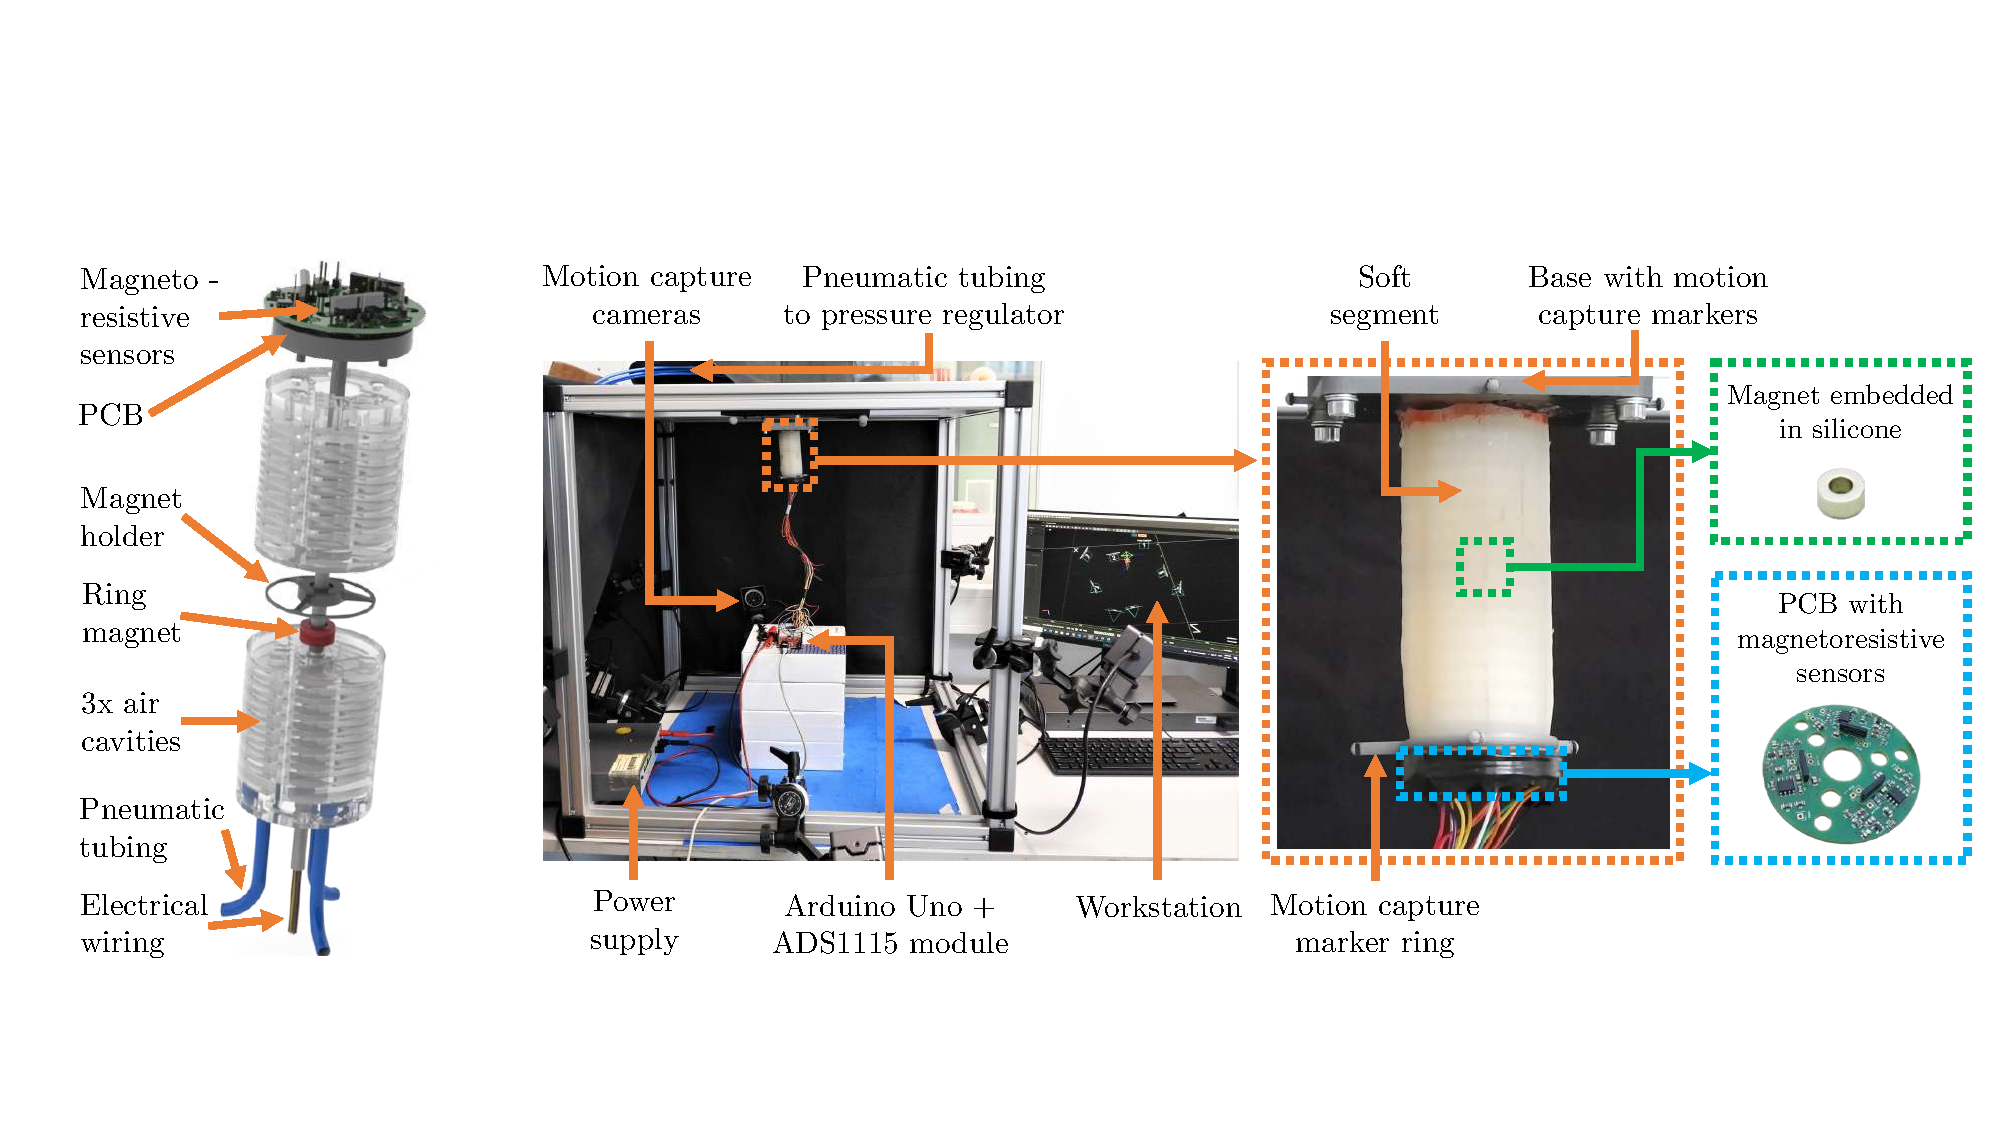
\includegraphics[width=1.0\textwidth]{promasens/figures/experimental_setup/experimental_setup_v5_compressed.pdf}
    \caption{
    \textbf{Left:} Exploded rendering visualizing the robot design with the three magnetoresistive sensors integrated into a PCB at the tip of the segment. The electrical wires from the PCB are passed through the backbone to the base. A ring magnet attached to a 3D-printed holder is integrated into the backbone at a half-segment-length distance from the proximal end. The air chambers of the segment are connected to a pressure regulator via tubing glued at the base of the segment. \textbf{Right:} Experimental setup with the soft robot segment attached in tip-down configuration to the motion capture cage.
    }\label{fig:promasens:experimental_setup}
\end{figure*}
% \begin{figure*}[hbt]
%     \centering
%     \subfigure[Design]{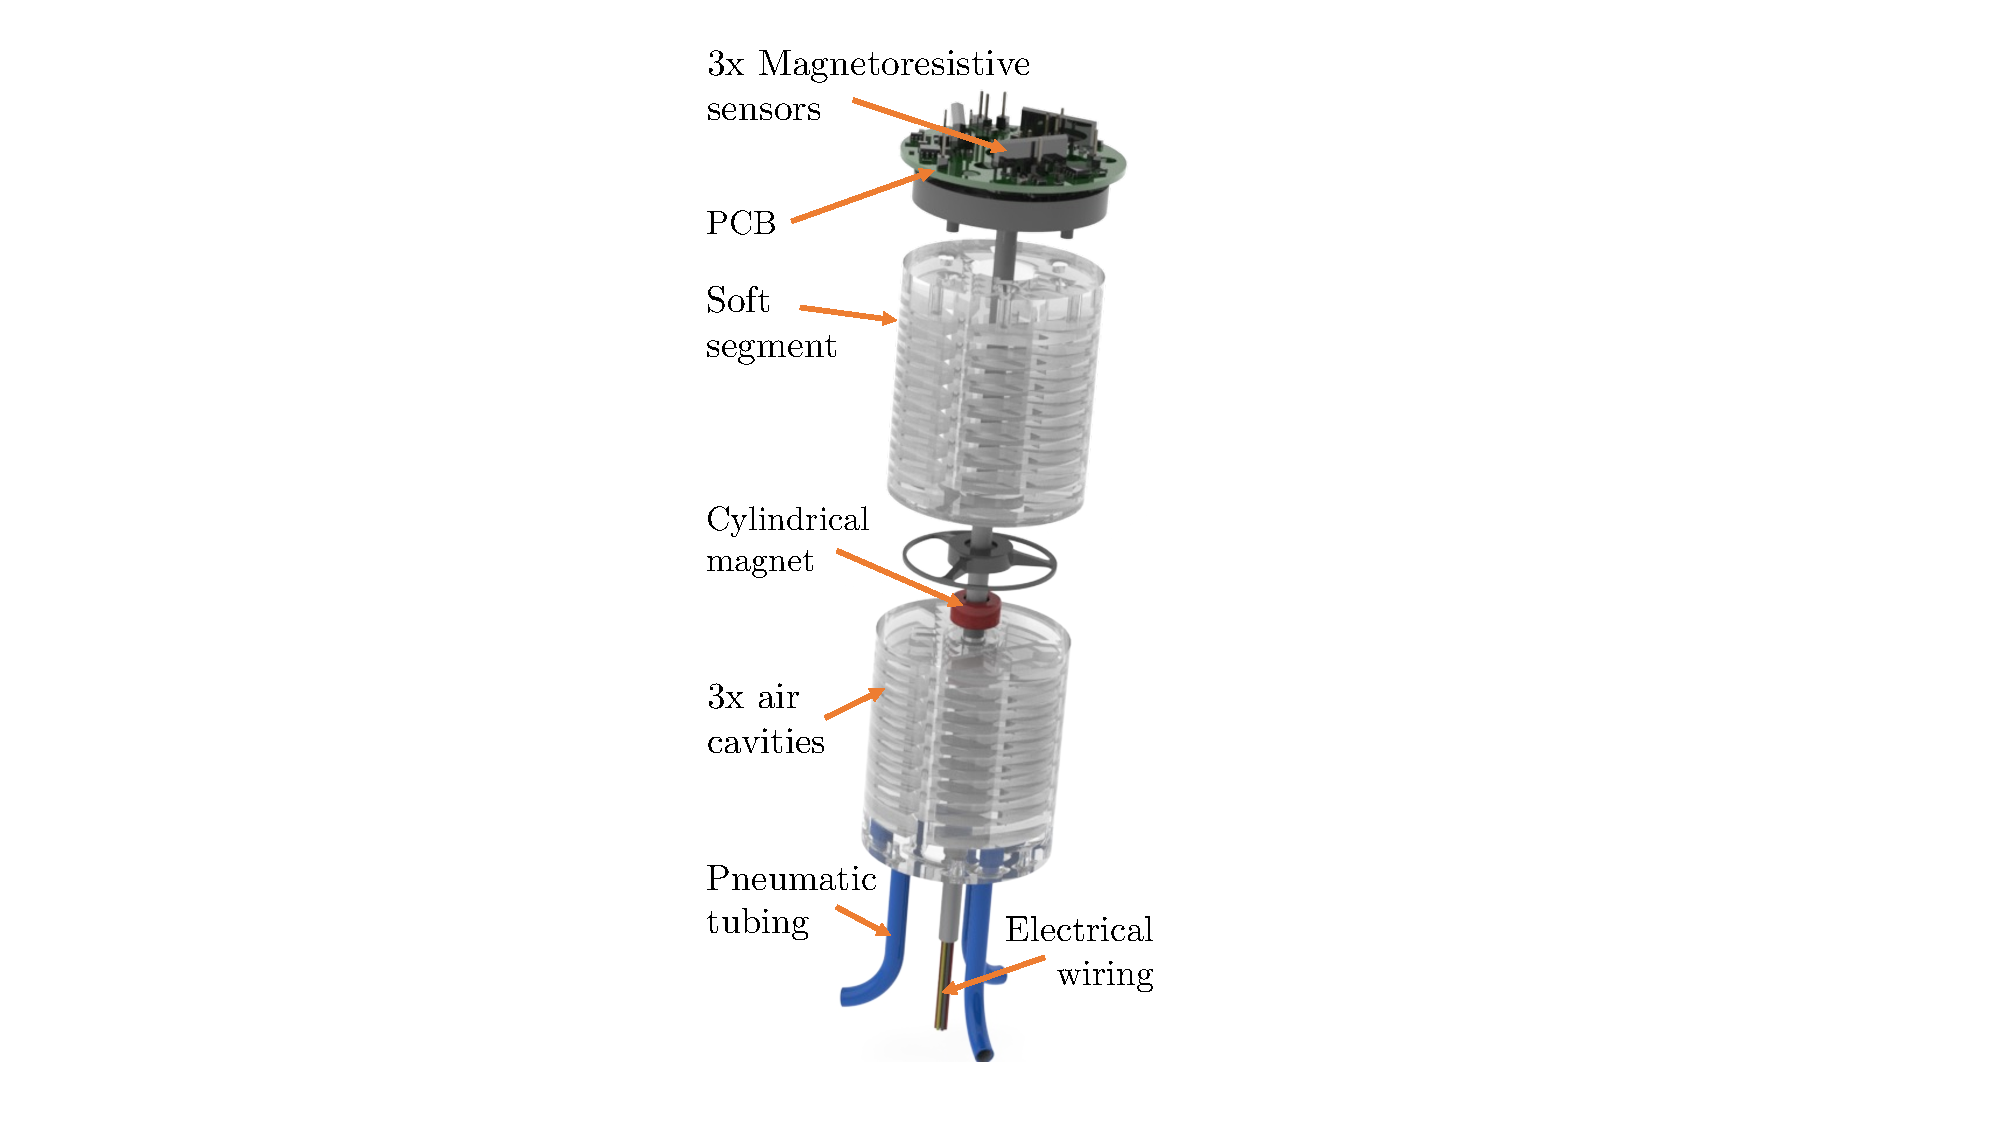
\includegraphics[width=0.135\textwidth]{promasens/figures/segment_design/segment_exploded_rendering_labeled_v1_cropped.pdf}\label{fig:promasens:exploded_rendering}}
    % \hspace{1pt}
%     \hfill
%     \subfigure[Experimental setup]{\includegraphics[width=0.65\textwidth]{promasens/figures/experimental_setup/experimental_setup_v4_compressed.pdf}\label{fig:promasens:experimental_setup}}
%     % \hspace{1pt}
%     \hfill
%     \subfigure[Actuated soft robot]{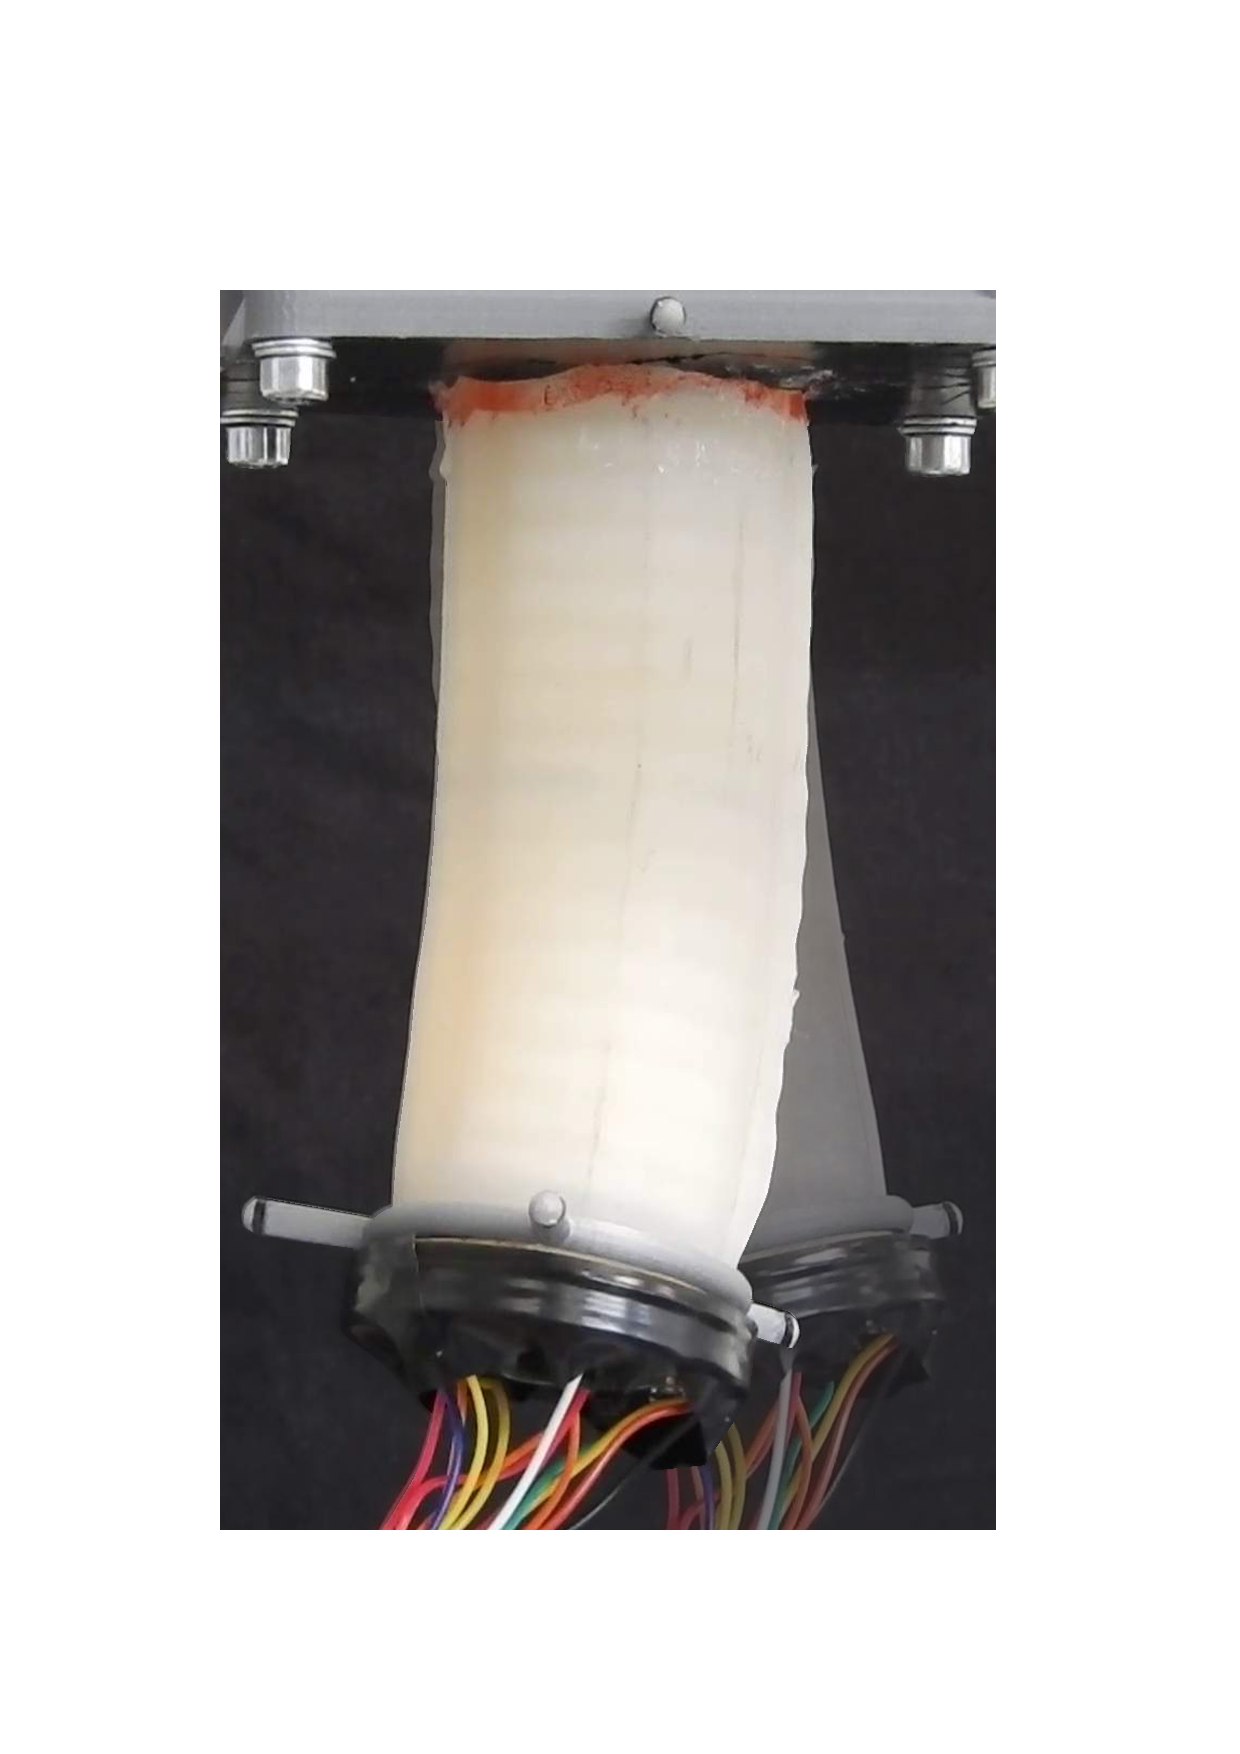
\includegraphics[width=0.16\textwidth]{promasens/figures/robot_bending/Overlapping_images_left_solid_right_transparent_compressed.pdf}\label{fig:promasens:actuated_soft_robot}}
%     \caption{\textbf{Panel (a):} Exploded rendering visualizing the robot design with the three magnetoresistive sensors integrated into a PCB at the tip of the segment. The electrical wires from the PCB are passed through the backbone to the base. A ring magnet attached to a 3D-printed holder is integrated into the backbone at a half-segment-length distance from the proximal end. The air chambers of the segment are connected to a pressure regulator via tubing glued at the base of the segment. \textbf{Panel (b):} Experimental setup with the soft robot segment attached in tip-down configuration to the motion capture cage. % Magnet and \gls{PCB} with \glsp{MRS} are scaled relative to the soft robot segment.
%     \textbf{Panel (c):} Evolution of a soft robot during 1D bending.}
% \end{figure*}

We verify the performance of our proposed proprioception method in experiments involving one soft robot segment with three magnetoresistive sensors attached to the tip.
We aim to estimate the CC configuration $\hat{q} = (\Delta_{x,1}, \Delta_{y,1})^\top \in \mathbb{R}^2$ from the measured sensor values $u(t) \in \mathbb{R}^3$.
% We collect a training set of random actuation sequences produced with \gls{GBN}~\citep{tulleken1990generalized}.
We let the robot follow a diverse set of trajectories and evaluate the proprioception performance.
After measuring the ground-truth pose of the tip of the segment with a motion capture system, we perform inverse kinematics with the closed-form solution reported by Della Santina et al.~\citep{della2020improved} and quantitatively compare the proprioceptive configuration estimate of the segment with the ground-truth configuration.

\begin{figure*}[hbt]
  \centering
  \subfigure[\textbf{T0:} random setpoints]{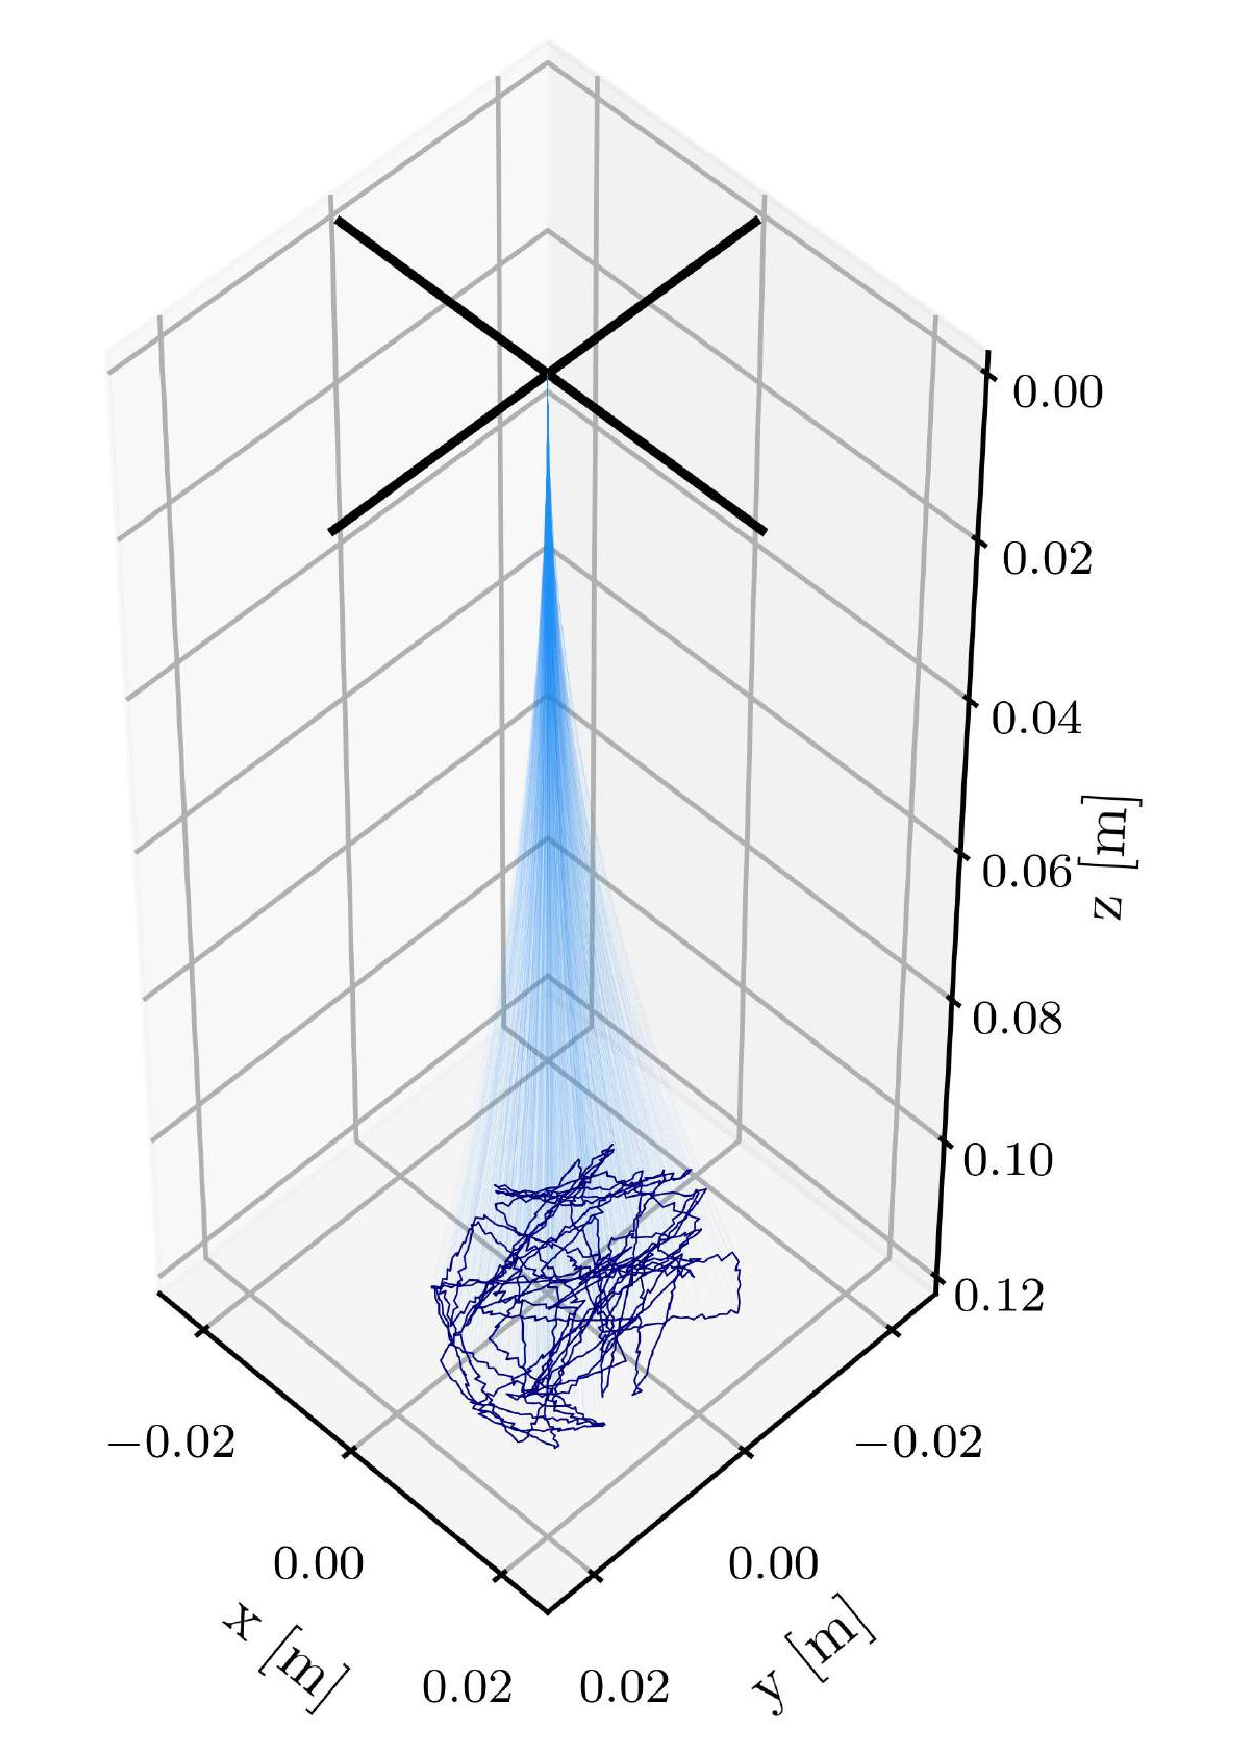
\includegraphics[width=0.16\textwidth]{promasens/figures/trajectories/trajectory_visualizations/random_compressed.pdf}}
  % \hfill% or \hspace{5mm} or \hspace{0.3\textwidth}
  \subfigure[\textbf{T1:} 1D bending]{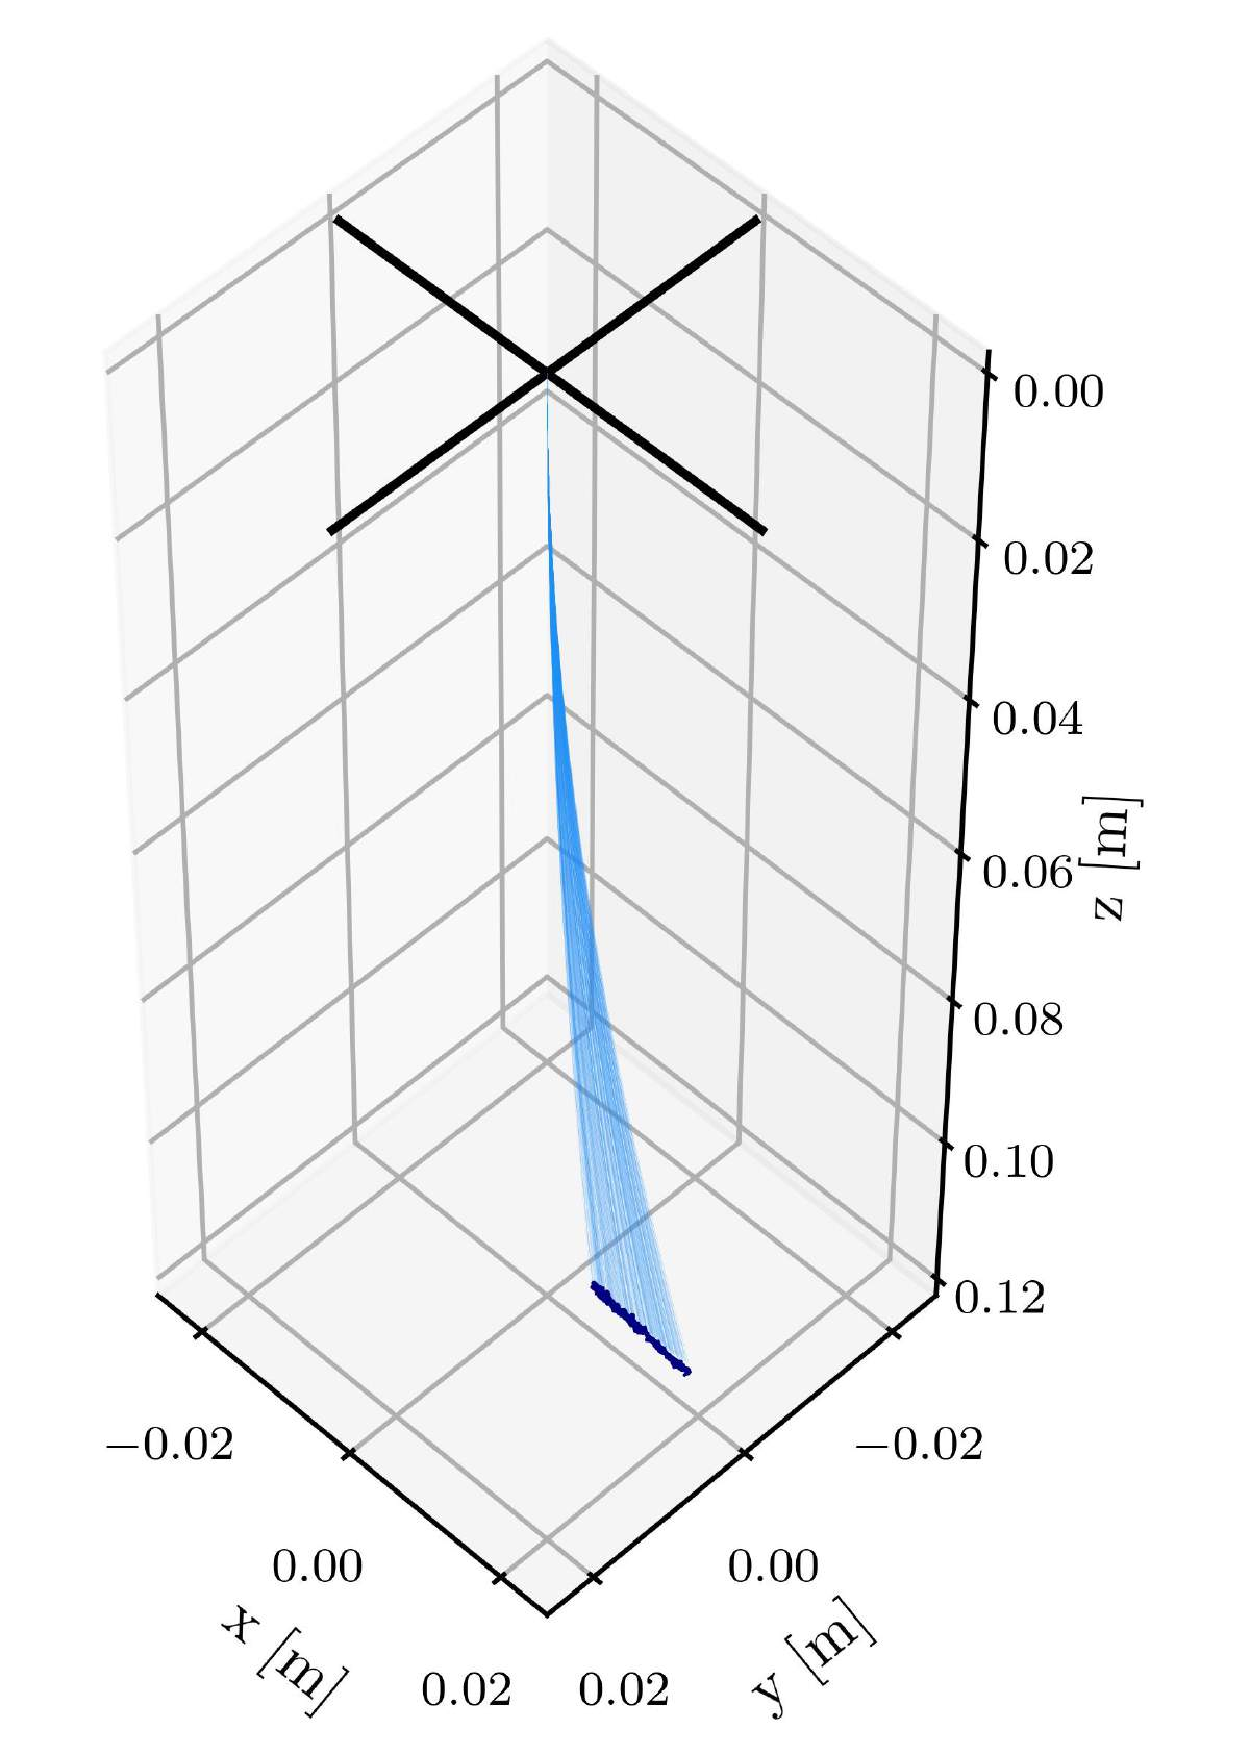
\includegraphics[width=0.16\textwidth]{promasens/figures/trajectories/trajectory_visualizations/1D_bending_compressed.pdf}}
  \subfigure[\textbf{T2:} half lemniscate]{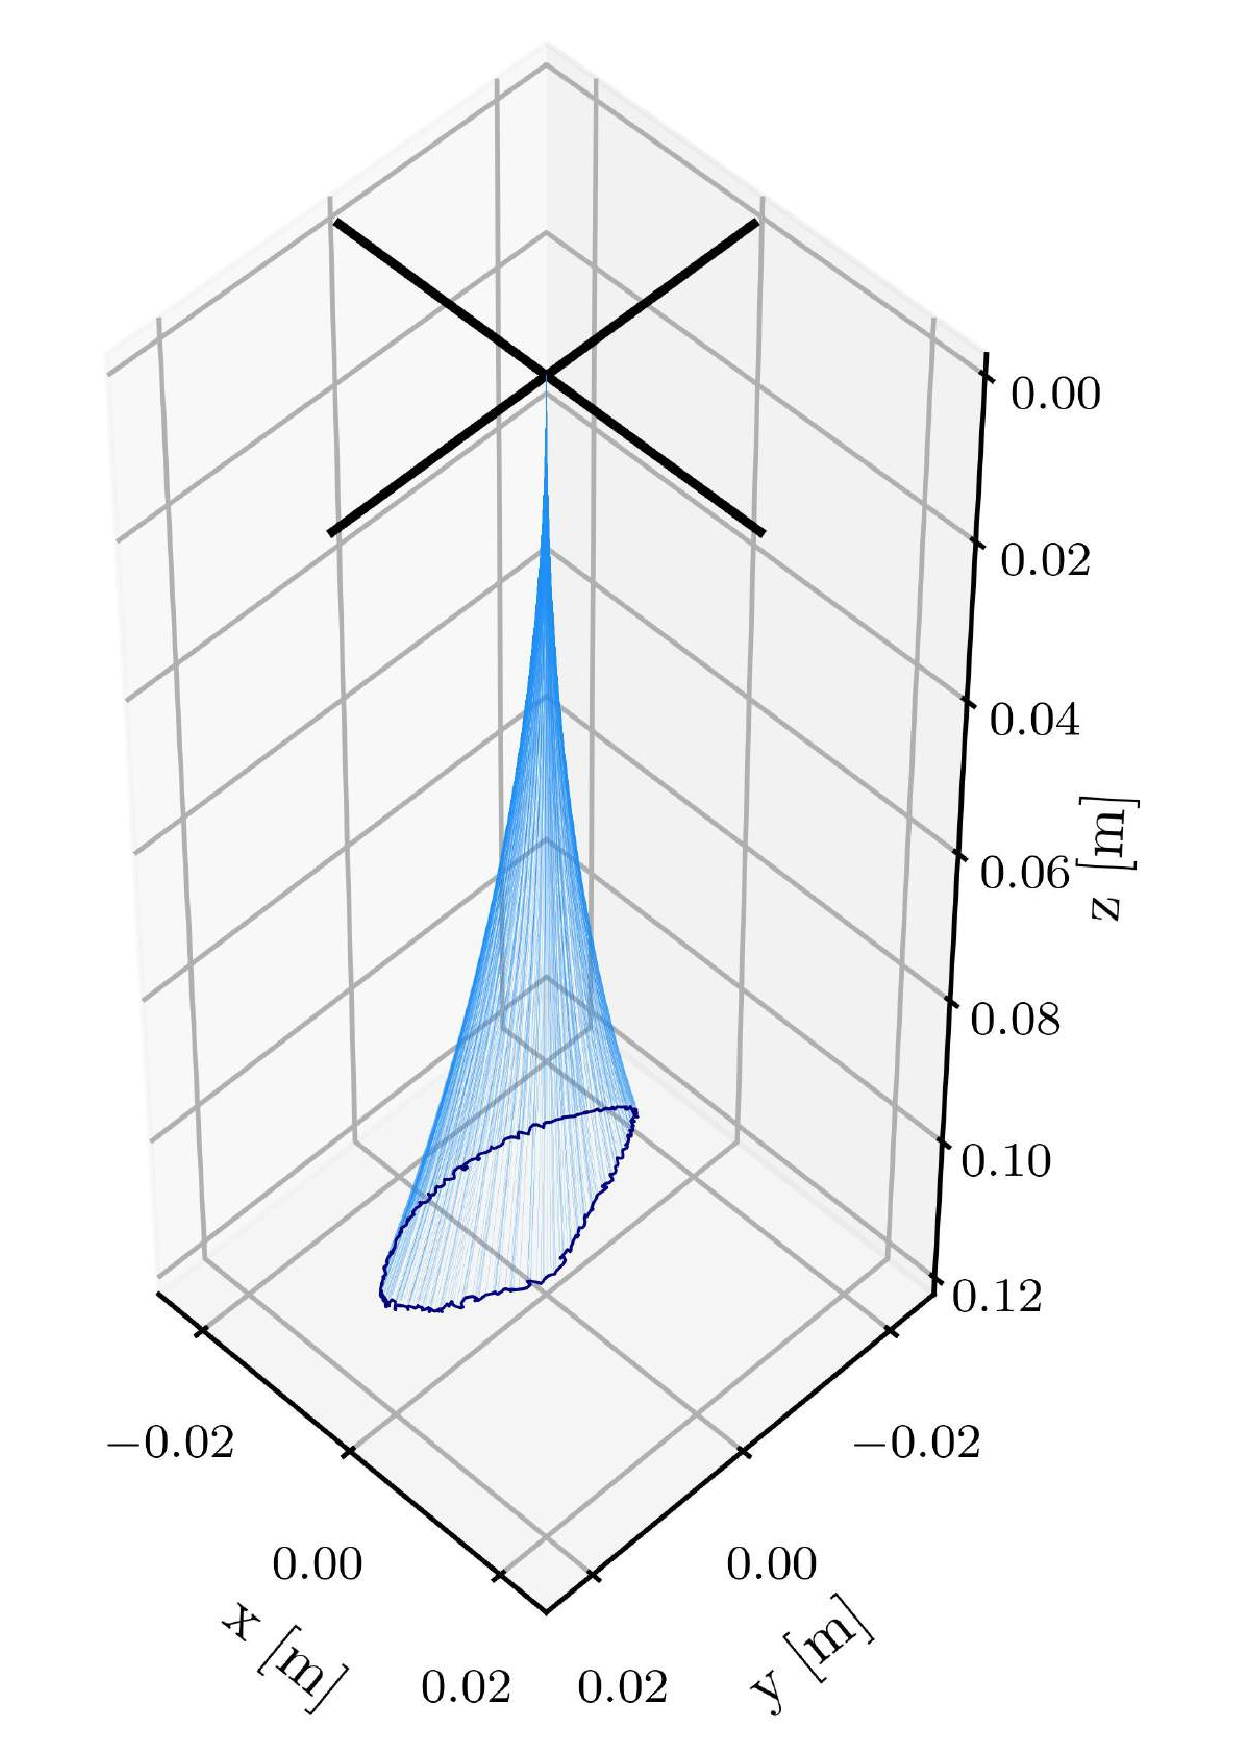
\includegraphics[width=0.16\textwidth]{promasens/figures/trajectories/trajectory_visualizations/half_lemniscate_compressed.pdf}}
  \subfigure[\textbf{T3:} full lemniscate]{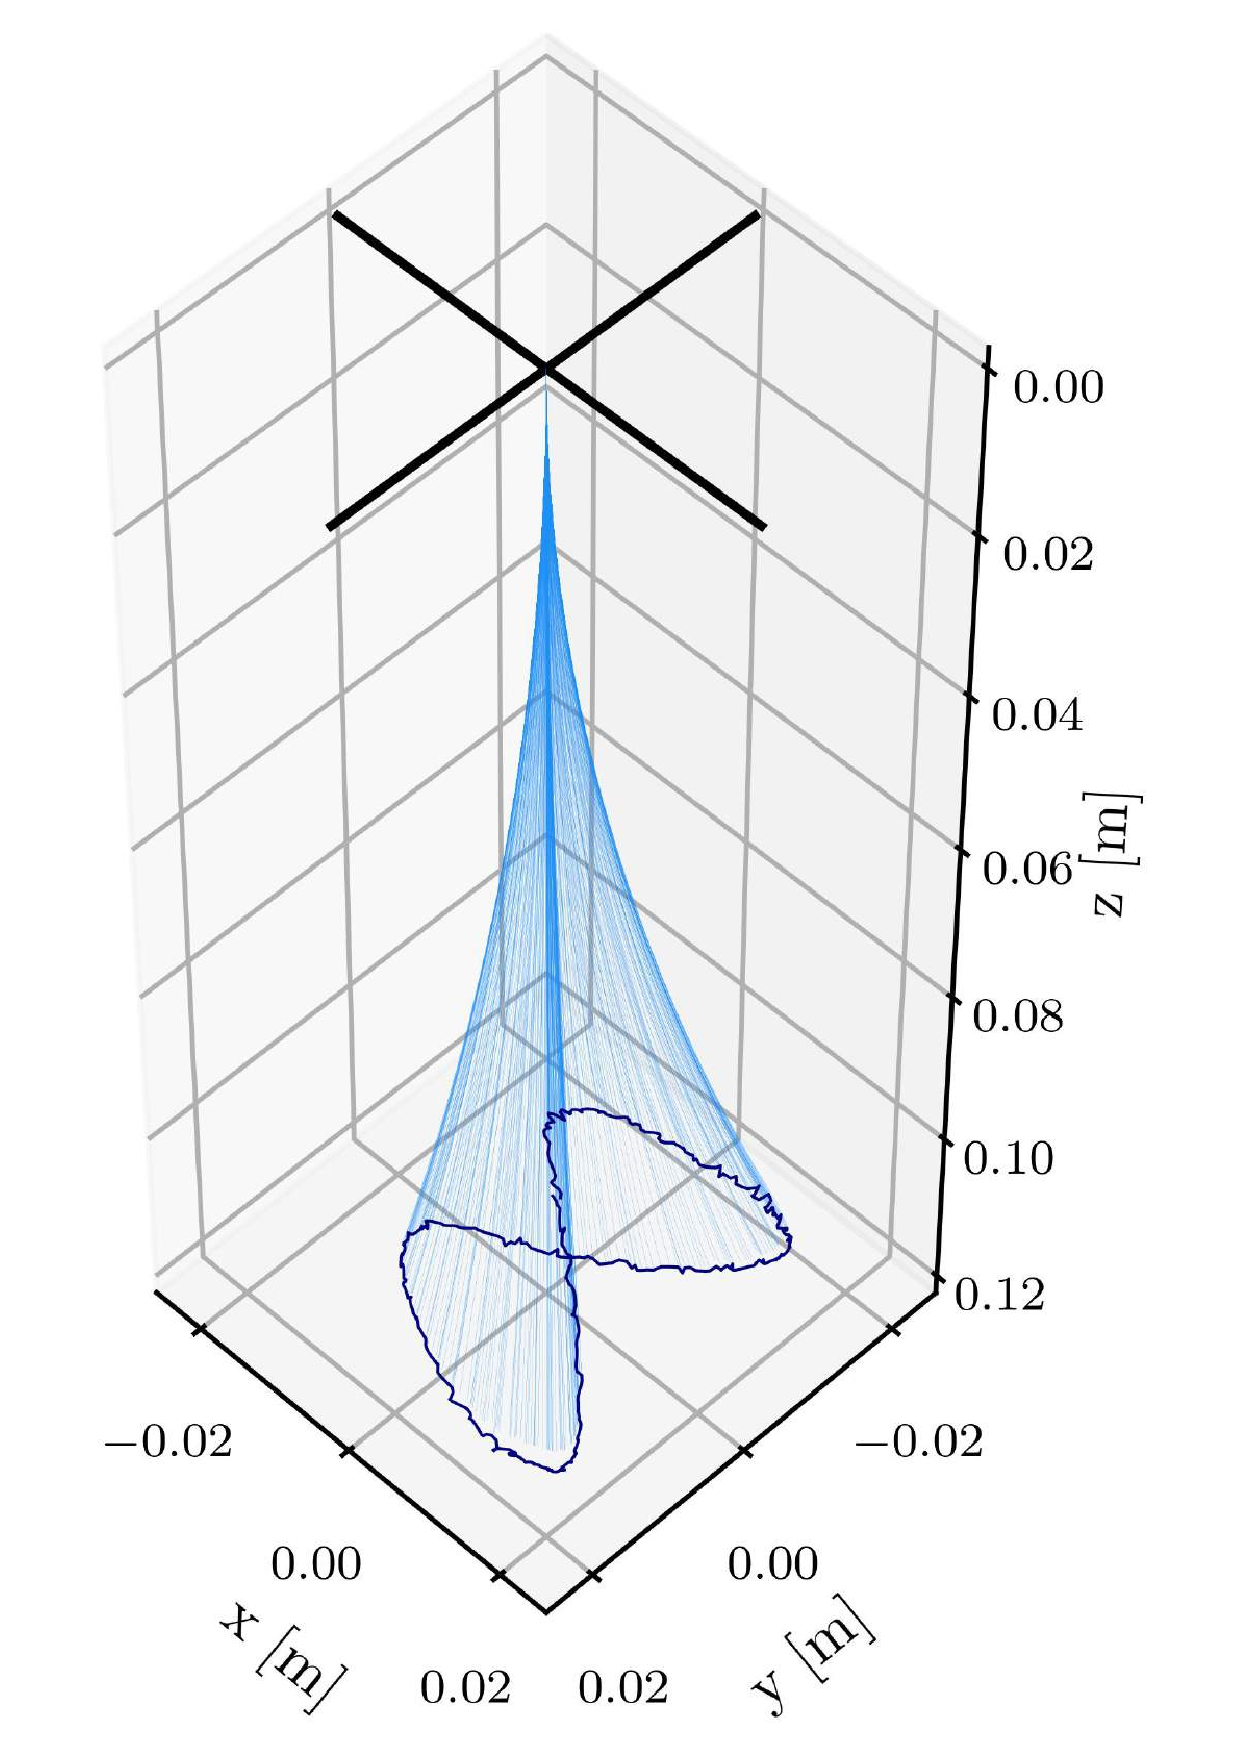
\includegraphics[width=0.16\textwidth]{promasens/figures/trajectories/trajectory_visualizations/full_lemniscate_compressed.pdf}\label{fig:promasens:t3_viz}}
  \subfigure[\textbf{T4:} spiral]{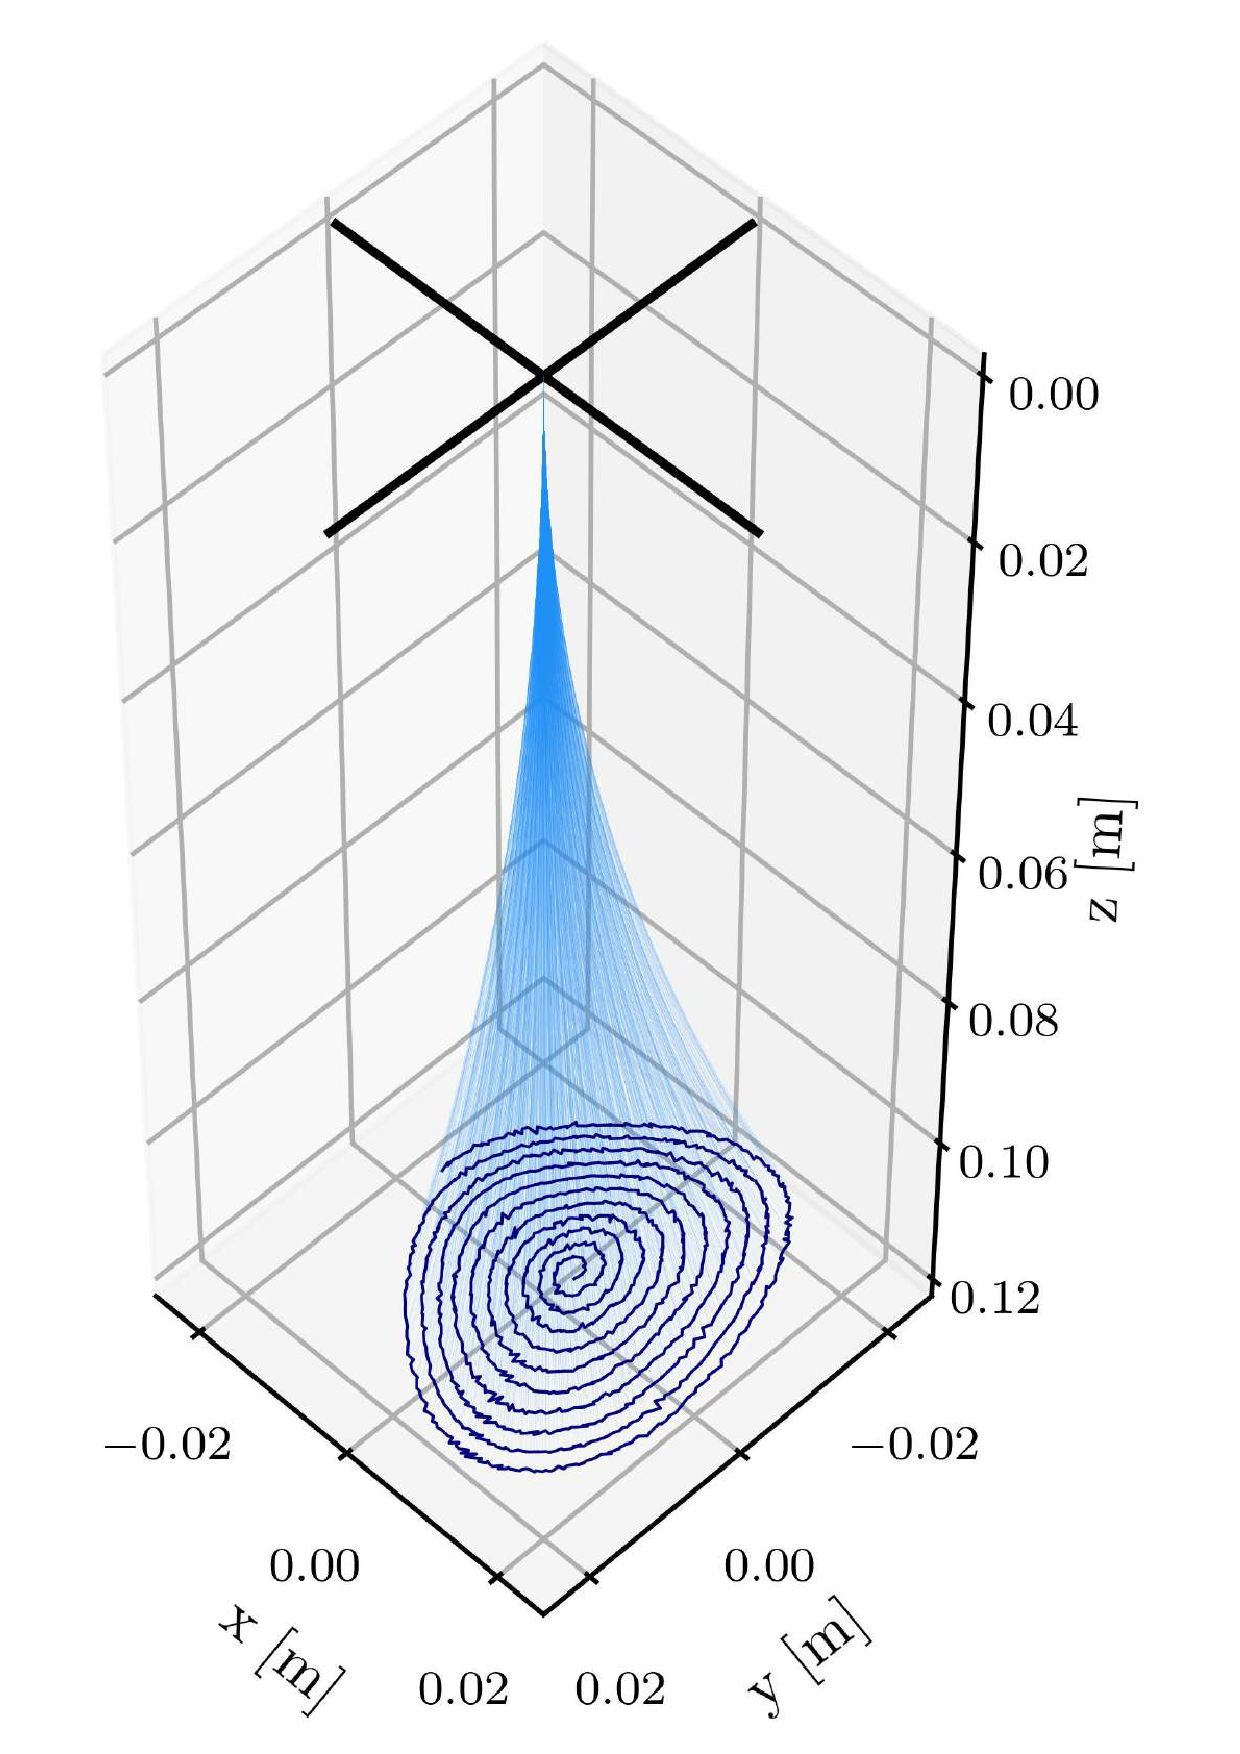
\includegraphics[width=0.16\textwidth]{promasens/figures/trajectories/trajectory_visualizations/spiral_compressed.pdf}}
  \subfigure[\textbf{T5:} flower]{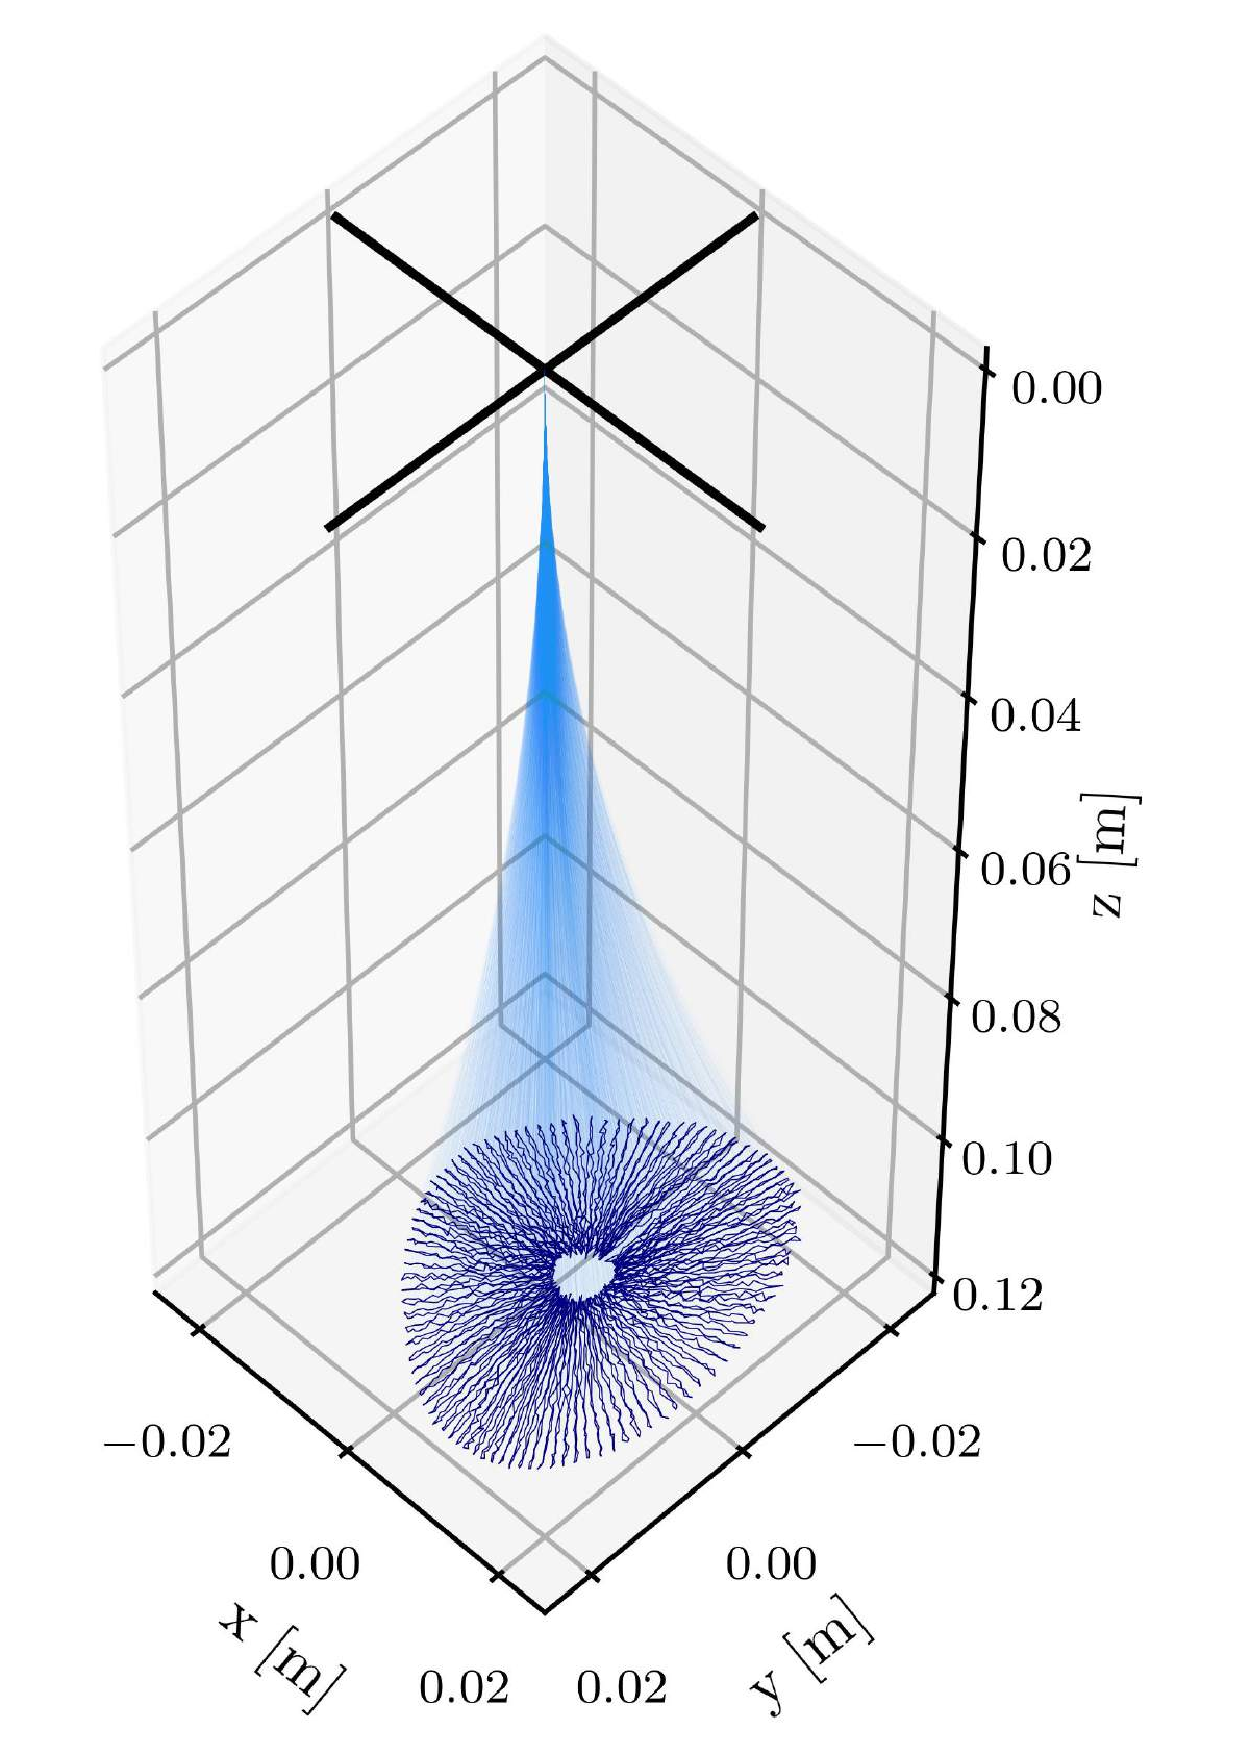
\includegraphics[width=0.16\textwidth]{promasens/figures/trajectories/trajectory_visualizations/flower_compressed.pdf}}
%   \hfill
%   \subfigure[Neural network architecture]{\includegraphics[width=0.33\textwidth]{promasens/figures/Experiments/NN_architecture_P.pdf}\label{fig:promasens:NNgradientdescent}}
  \caption{Trajectories used during the experiments. We plot the shape of the segment under \gls{PCC} approximation in light blue and the position of the tip of the segment in dark blue. 
  % Trajectory 1 represents a 1D bending, trajectory 2 a half lemniscate, trajectory 3 a full lemniscate movement of the tip and trajectory 4 resembles a spiral. 
  % \textbf{Panel (e):} Architecture of the sensor measurement prediction network. Each block consists of a linear layer, a \gls{ReLU}, and a batch norm layer.
  }
  \label{fig:promasens:trajectories}
\end{figure*}

\subsection{Robot design}\label{sub:promasens:robot_design}
We use a cylindrical, pneumatically-actuated soft robotic silicon segment of length $L_{0}=\SI{110}{mm}$ and radius $d_1 = \SI{22}{mm}$ consisting of three independently inflatable cavities evenly spaced in the radial direction from the center line~\citep{marchese2015recipe}. 
% The robot is pneumatically actuated by adjusting the air pressure in each chamber to make the end-effector bend in 3D Cartesian space.
%
The proprioceptive sensing system is achieved by embedding one ring magnet in the backbone at a distance $d_{\mathrm{m}_0} = \SI{55}{mm}$ from the base of the segment and three symmetrically-placed Magnetoresistive Sensors (MRSs) at the tip of the segment as visualized in Fig.~\ref{fig:promasens:experimental_setup}. % Fig.~\ref{fig:promasens:exploded_rendering}.
Although we use MRSs in our experimental setup for their high sensitivity~\citep{popovic2002bridging}, this is not a strict condition and other sensor types measuring the magnetic field such as Hall-effect sensors can be combined with the methodology proposed in this chapter too.
For casting the silicone segment, we use a 3D-printed mold with a holder for the magnet which keeps it in place inside the segment.
The magnet used is a neodymium ring of grade N50 with a thickness and inner diameter of \SI{6}{mm} each, and an outer diameter of \SI{12}{mm}.
%
The MRSs of type Honeywell HMC1021Z are integrated into a Printed Circuit Board (PCB) and output a voltage difference of \SI{50}{mV \per mT}. % ~\citep{honeywell}. 
The three sensors are equally spaced at \SI{120}{\degree} from each other and are placed at a radial distance of $d_{\mathrm{s},\mathrm{r}} = \SI{13}{mm}$, and at a longitudinal distance of $d_{\mathrm{s},\mathrm{a}} = \SI{116}{mm}$ from the base in a straight configuration.
For each sensor, we implemented a Set / Reset and an amplification circuit on the PCB.
The Set / Reset circuit is used for calibration of the sensor by re-aligning the magnetic domains. After amplification of the sensor output by a factor of 100, the output of the sensors is processed with a Texas Instruments ADS1115 module %~\citep{ADS1115module}
resulting in a digital signal of \SI{16}{bit} resolution. All sensor measurements $u$ are in the range $[\SI{0}{mV}, \SI{2048}{mV}]$, which corresponds to magnetic flux densities of  $[\SI{0}{mT}, \SI{41}{mT}]$.

%The \gls{MRS} are mounted on a \gls{PCB} at the tip of the silicone body, with three sensors on one PCB. The exact placement of the sensors is shown in Table \ref{tab:sensor_locations}. The sensors are Honeywell HMC1021Z sensors that have an ideal operating range of $\SI{\pm 6}{Gs}$. The sensor gives a voltage difference of \SI{5}{mV \per Gs} as an output \citep{honeywell,farnell}.
%
% The \gls{PCB} is mounted on either side of the silicone body. The holes in the \gls{PCB} are for the air supply hoses, cables, and mounting. The \gls{PCB} not only contains the sensors, but also the sensor circuitry. Each sensor has its own circuitry containing a Set/Reset circuit and an amplification circuit. The Set/Reset circuit produces a current peak of \SI{1}{A} of duration $\SI{2}{\micro \second}$ for a Set/Reset pulse to calibrate the sensor by realigning the magnetic domains in the sensor in one direction. The amplification circuit amplifies the sensor output by a factor of 100. The output of the sensors is processed with a Texas Instruments ADS1115 module \citep{ADS1115module}. This module reads out the sensor signal in 16 bits and fits it into a format so that the Arduino can read it out. This gives a more precise sensor readout than using the Arduino directly which would only give a \SI{10}{bit} resolution.\\

% Fabrication
% The fabrication process of the silicone body starts by making three wax inserts by pouring beeswax into a silicone mold. Once hardened, these wax inserts are removed from their silicone mold and placed into a 3D-printed mold together with the magnet holder. The magnet holder is a 3D-printed ring that houses the magnet. Subsequently, Dragon Skin 30 silicone is mixed, degassed, and poured into the 3D-printed mold. After hardening, the silicone body, wherein the magnet holder and magnet are embedded, is removed from the mold. Then the wax inserts are melted, leaving three inflatable chambers behind.

% \begin{figure}[ht]
% \centering
% \includegraphics[width=50mm]{promasens/figures/PCB_3d_view_2.png}
% \caption{\gls{PCB} for three \gls{MRS} including Set/Reset circuit to be mounted at the base and tip of each segment.}\label{fig:promasens:PCB}
% \end{figure}
        

\begingroup
\setlength{\tabcolsep}{6pt} % Default value: 6pt
\begin{table*}\footnotesize
\centering
\caption{Experimental results: absolute [mm] and relative RMSE [\%] of sensor measurement predictions and robot configuration estimates for various trajectories. The RMSE is normalized with the range of the dataset for $u$ and each configuration variable respectively as stated in \eqref{eq:promasens:relative_RMSE}. We report the error as $\text{mean} \pm \text{stdev}$ and compute the statistics over three different random seeds. The random seed determines at the start of the training the initialization of the neural network weights.}
\begin{tabular}{l rr rrrr}\toprule
\textbf{Trajectory} & $e_{u}$ [mV] & $e_{u}$ [\%] & $e_{\Delta_x}$ [mm] & $e_{\Delta_x}$ [\%] & $e_{\Delta_y}$ [mm] & $e_{\Delta_y}$ [\%]\\
\midrule
T5.train $\rightarrow$ T0.test & $9.90 \pm 0.90$ & $3.90 \pm 0.40$ & $0.37 \pm 0.06$ & $3.70 \pm 0.60$ & $0.44 \pm 0.01$ & $3.50 \pm 0.10$\\ % T5.slow_to_T0.200mBar
T5.train $\rightarrow$ T1.test & $8.80 \pm 0.30$ & $4.40 \pm 0.10$ & $0.36 \pm 0.08$ & $6.50 \pm 1.50$ & $0.43 \pm 0.05$ & -\\ % T5.slow_to_T1.270
T5.train $\rightarrow$ T2.test & $11.10 \pm 0.30$ & $4.30 \pm 0.10$ & $0.78 \pm 0.03$ & $13.60 \pm 0.60$ & $0.74 \pm 0.23$ & $5.90 \pm 1.80$\\ % T5.slow_to_T2
T5.train $\rightarrow$ T3.test & $12.30 \pm 0.30$ & $4.60 \pm 0.10$ & $0.52 \pm 0.06$ & $4.50 \pm 0.50$ & $0.47 \pm 0.03$ & $3.10 \pm 0.20$\\ % T5.slow_to_T3_90deg
T5.train $\rightarrow$ T4 & $3.01 \pm 0.05$ & $1.08 \pm 0.02$ & $0.33 \pm 0.02$ & $2.40 \pm 0.10$ & $0.52 \pm 0.06$ & $3.10 \pm 0.40$\\ % T5.slow_to_T4.slow.forw
T5.train $\rightarrow$ T5.test & $1.60 \pm 0.10$ & $0.58 \pm 0.05$ & $0.24 \pm 0.05$ & $1.90 \pm 0.30$ & $0.24 \pm 0.01$ & $1.40 \pm 0.05$\\ % T5.slow_to_T5.slow
\bottomrule
\end{tabular}
\label{tab:results_experiments}
\end{table*}
\endgroup

\subsection{Experimental setup}
We conducted our experiments in a lab environment with the base of the soft robot segment mounted in a tip-down configuration to a cubical cage as shown in Figure~\ref{fig:promasens:experimental_setup}.
% Motion Capture System
A 3D-printed ring with four reflective markers is mounted on the tip of the segment.
% Prime X by Optitrack
Eight motion capture cameras are attached to the cage tracking at \SI{40}{Hz} the 3D pose of the ring.
We transform the pose measurements of the tip to the base frame of the robot and compute the closed-form inverse kinematics~\citep{della2020improved} to receive a ground-truth configuration estimate $q(t) \in \mathbb{R}^2$.
% Pneumatic actuation
Each of the three pneumatic chambers of the segment is connected via tubing to a separate valve of a proportional pressure regulator operated at \SI{100}{Hz}. % We send set-point pressure commands from the workstation to the pressure regulator via Modbus / TCP at \SI{100}{Hz}.
% Reading sensor measurements
We read out the analog signals of the magnetoresistive sensors with an Arduino Uno at \SI{40}{Hz} and save them for later offline processing. 
We temporally align the motion capture and the magnetic sensor data by detecting the initial extension of the robot with a suitable threshold.
%static distortion
The sensor noise is determined for both an unelongated straight configuration, and during fully inflated bending. Here the standard deviations of the white noise are \SI{0.24}{mV} and \SI{3.55}{mV}, which normalizes to \SI{0.03}{\percent} and \SI{2}{\percent} of the dynamic range respectively.
% earth's magnetic field
% Furthermore, we measure the angle between the x-axis of the base frame and the magnetic north with a compass as $\varphi_\mathrm{e} = \SI{3.79}{\radian}$ and rely on the \gls{WMM}~\citep{chulliat2020us} to identify the vertical component of the earth's magnetic field. This results in a unit vector for the earth's magnetic field direction of $\{ \hat{n}_{\mathrm{e}} \}_{0} = (-0.311, -0.234, 0.921)^\top$ for the robot in tip-down configuration.
Furthermore, we identify the earth's magnetic field direction in the base from as $\{ \hat{n}_{\mathrm{e}} \}_{0} = (-0.311, -0.234, 0.921)^\top$ using a compass and the World Magnetic Model (WMM)~\citep{chulliat2020us}.

\begin{figure*}[hbt]
  \centering
  \subfigure[Loss landscape]{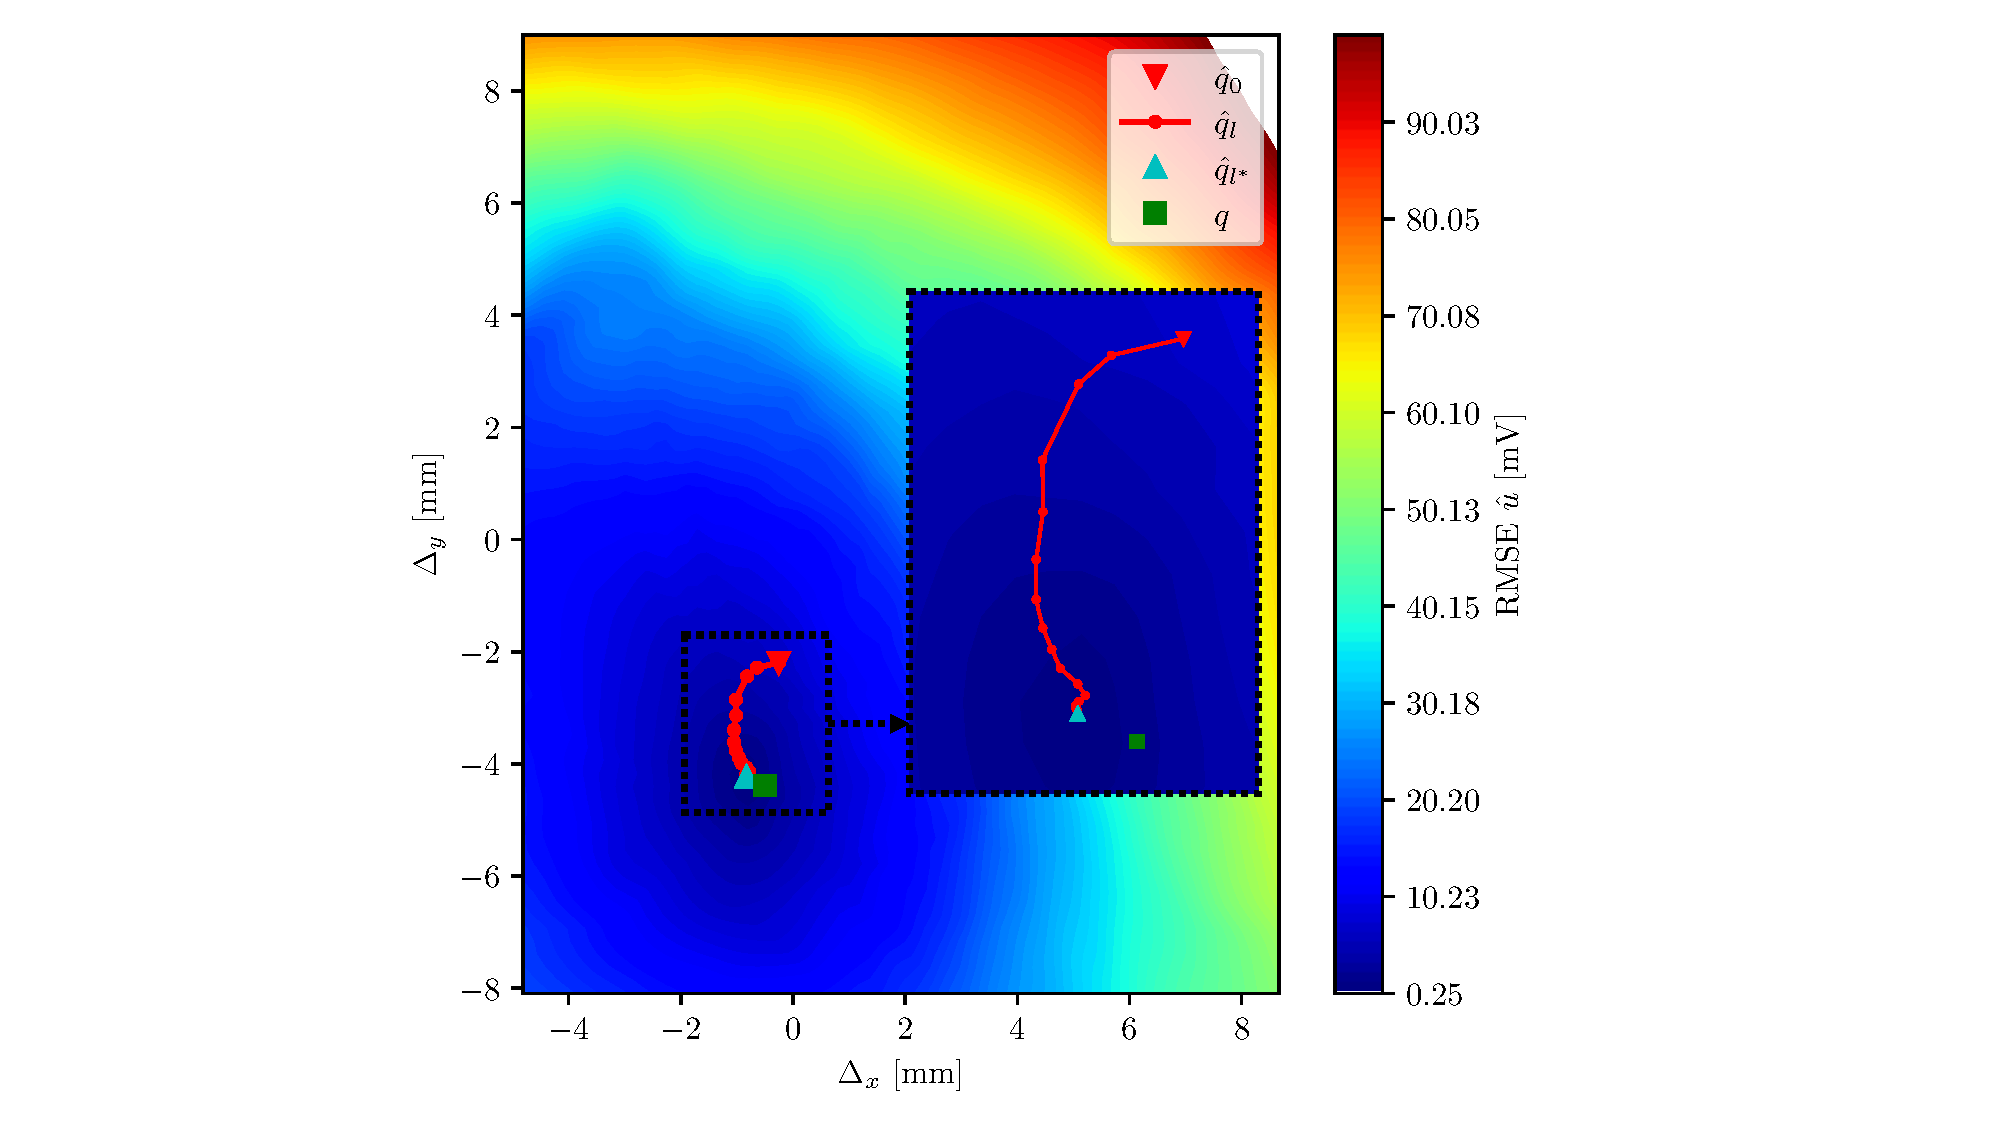
\includegraphics[width=0.3125\textwidth]{promasens/figures/loss_landscape/loss_landscape_v3_cropped.pdf}\label{fig:promasens:loss_landscape}}
  %
  \subfigure[Experimental results for T2 (top) and T5 (bottom)]{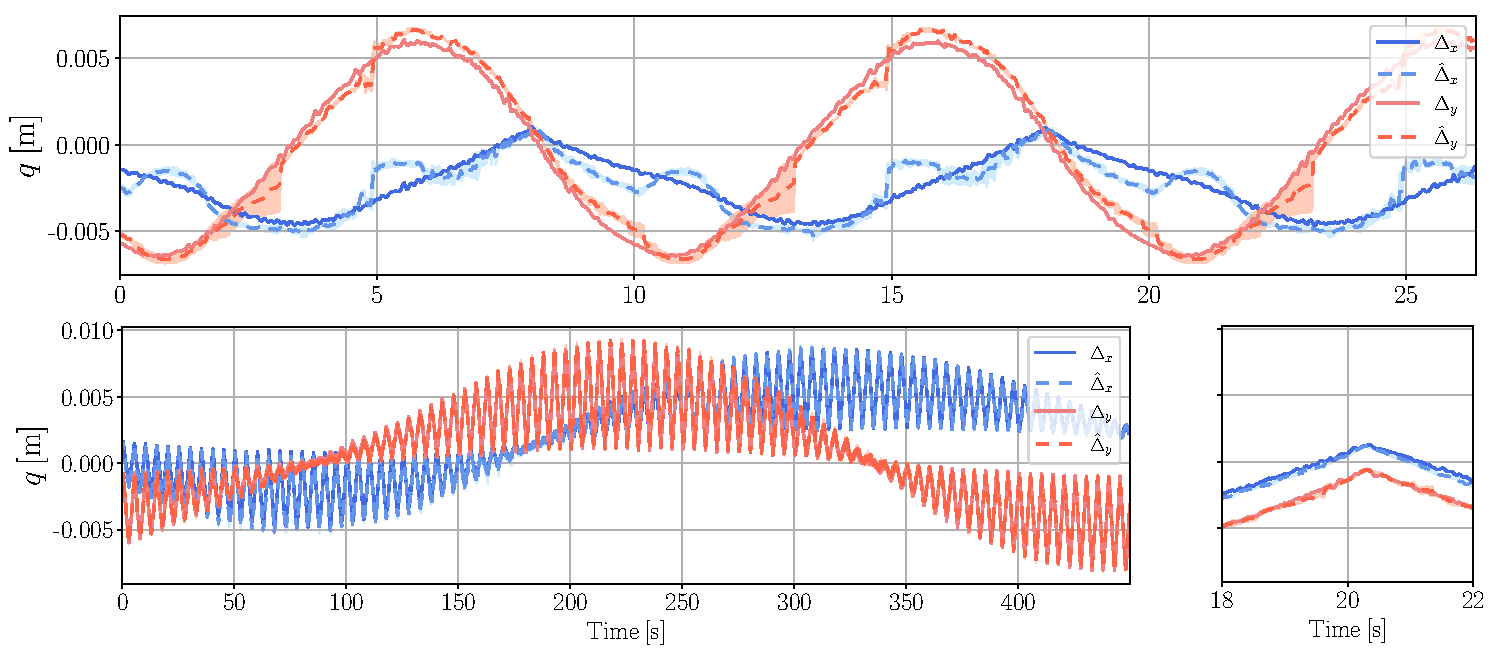
\includegraphics[width=0.6775\textwidth]{promasens/figures/experimental_results/2022-05-02_results_merged.pdf}\label{fig:promasens:2022-05-02_results_merged}}\\ %  [T5.train $\rightarrow$ T2.test] [T5.train $\rightarrow$ T5.test]
  
  \caption{\textbf{Panel (a):} Sample loss landscape for optimization of $\Delta_x$ and $\Delta_y$ on T5. With the hue, we visualize the RMSE of the sensor measurement prediction $\hat{u}$ for a given configuration $\hat{q} = (\Delta_x, \Delta_y)^\top$. Additionally, we denote the initial configuration estimate with $\hat{q}_0$, the trajectory of the gradient descent with $\hat{q}_l$, the optimal configuration with $\hat{q}$, and the ground truth with $q$. \textbf{Panel (b) top:} Proprioception on the test set of T2 using a model trained on T5. \textbf{Panel (b) bottom:} Configuration estimates for a model trained and evaluated on separated parts of trajectory 5. We plot the ground-truth configuration $q$ in solid, the estimate $\hat{q}$ as a mean over three random seeds with dashed lines, and the standard deviation as an error band. The bottom right plot zooms onto a selected part of T5 (e.g. \SI{18}{s} to \SI{22}{s}) to more clearly visually distinguish the dashed lines from the solid lines.}
  \label{fig:promasens:results_trajectories}
\end{figure*}

\subsection{Pneumatic actuation and trajectories}
% We consider two actuation sequence types in this chapter: a) a randomized actuation sequence consisting of steps generated with \gls{GBN}~\citep{tulleken1990generalized} primarily used for training and b) three continuous trajectories consisting of planar side bending, and the tip following half-8-shape and full 8-shapes as plotted in Fig.~\ref{fig:promasens:trajectories}.
We consider, as visualized in Fig.~\ref{fig:promasens:trajectories}, six continuous actuation sequences in this chapter: random configuration way-points which are connected through linear interpolation (T0), planar side bending (T1), the tip following a half lemniscate (T2) and full lemniscate (T3), a spiral with constant linear velocity~\citep{carrasco2018constant} (T4) and finally a flower-shape (T5).
We define our trajectories as wrenches  $\tau_\mathrm{xyz} = \begin{bmatrix} \tau_\mathrm{x} & \tau_\mathrm{y} \end{bmatrix}^\top$ on the tip of the segment in Cartesian space, where $\tau_\mathrm{x}$ and $\tau_\mathrm{y}$ cause bending around the local x- and y-axis  of the tip respectively. % $f_\mathrm{z}$ is a force leading the segment to extend uniformly.
The pressures we command from the pressure regulator are given by inversely evaluating the force produced at the center of pressure at the tip of the segment for each chamber for a given chamber pressure~\citep{della2019dynamic}.
All actuation sequences are preceded by first applying an offset pressure of \SI{225}{mBar} in all chambers, which causes a near-constant elongation of the segment. The peak pressure, which causes maximum bending, is set for all trajectories to \SI{450}{mBar}.

% The \gls{GBN}~\citep{tulleken1990generalized} algorithm with an expected settling time of \SI{5}{s} determines the timing of when we command a step to a new random wrench $\tau_{xzy}$.
% We uniformly sample a bending azimuth angle $\varphi \sim \mathcal{U}\left(0, 2 \pi\right)$, a bending torque magnitude $|\tau| \sim \mathcal{U}\left(0, \tau_\mathrm{max}\right)$ and accordingly compute $\tau_\mathrm{xyz}$ as
% \begin{equation}
%     \tau_\mathrm{x} = \cos(\varphi) |\tau| \qquad \tau_\mathrm{y} = \sin(\varphi) |\tau|
% \end{equation}
% and set $f_\mathrm{z}$ to a constant force with corresponding symmetric pressure of \SI{200}{mBar} in the chambers. The maximum bending torque $\tau_\mathrm{max}$ corresponds to a peak pressure in the chambers of \SI{425}{mBar}

% The planar side bending, half lemniscate, and full lemniscate trajectories are generated with a recurring linear torque increase/decrease sequence up to a peak pressure of \SI{425}{mBar}.
% Each T1-T3 trajectory is repeated six times to extend the length of the dataset.
% The spiral trajectory consists of linearly increasing the torque amplitude from a peak pressure of \SI{305}{mBar} to \SI{425}{mBar} over a duration of \SI{110}{s} while at the same time tracking a circular motion with an angular velocity of \SI{1.26}{rad/s}. In the second half of the trajectory, which is later used as a test set, the peak pressure is accordingly linearly decreased over time.

%The spiral trajectory consists of linearly increasing the torque amplitude from a peak pressure of \SI{305}{mBar} to \SI{425}{mBar} over a duration of \SI{110}{s} while at the same time tracking a circular motion with an angular velocity of \SI{1.26}{rad/s}. In the second half of the trajectory, which is later used as a test set, the peak pressure is accordingly linearly decreased over time. 

%The first part is generated with
%\begin{equation}
%    \tau_\mathrm{x} = \frac{2 t}{n_\mathrm{t}} \sin(2 \pi f t) \,     \tau_\mathrm{max} \qquad \tau_\mathrm{y} = \frac{2        t}{n_\mathrm{t}} \sin(2 \pi f t) \, \tau_\mathrm{max},
%\end{equation}
%where $f=\SI{0.2}{Hz}$ represents the frequency, and $\tau_\mathrm{max}$ the peak bending torque of the trajectory with a corresponding peak pressure of \SI{410}{mBar} in the chambers. We denote with $t$ the time and $n_\mathrm{t}$ the duration of the trajectory.

%Very similarly, we generate the planar side bending, half-8-shape, and full-8-shape trajectories with a recurring linear torque increase/decrease sequence up to a peak pressure of \SI{410}{mBar}.
%Each T1-T3 trajectory is repeated six times to extend the length of the dataset.

% We generate the planar side bending, half-8-shape, and full 8-shape trajectories with the following function:
% \begin{equation}
%     \tau_\mathrm{x} = A_x \sin(2 \pi F_x f t) \tau_\mathrm{max} \qquad \tau_\mathrm{y} = A_y \sin(2 \pi F_y f t) \tau_\mathrm{max}
% \end{equation}
% with an offset pressure of \SI{200}{mBar} causing a constant extension of the segment, $f$ representing the trajectory frequency, $\tau_\mathrm{max}$ the peak bending torque of the trajectory with a corresponding peak pressure of \SI{410}{mBar} in the chambers and $t$ the trajectory time.
% Duration of $n_\mathrm{t}=\SI{3.8}{s}$
% \textcolor{red}{TODO: fix this}
% We choose $F_x$, $F_y$, $A_x$, and $A_y$ appropriately to generate the different trajectories, which we report in Tab.~\ref{tab:trajectory_params}.

The 1D bending (T1), half lemniscate (T2) and full lemniscate (T3) are all executed periodically with a period of \SI{5}{s}, \SI{10}{s}, and \SI{10}{s} respectively. 
Trajectories T0 and T4 are characterized by a constant velocity in torque-space of \SI{0.025}{Nm \per s} and \SI{0.0125}{kNm \per s} respectively.
The flower trajectory T5 can be described as periodic 1D bending with a linearly changing azimuth angle. It exhibits an angular velocity of \SI{0.0126}{rad \per s} and a period of \SI{10}{s} for the bending, which results in $50$ bending cycles per circumnavigation.
While the random configuration setpoints of T0 are recorded for \SI{200}{s}, T1, T2 and T3 have total a duration of \SI{90}{s} each, and the spiral T4 and flower T5 last for \SI{120}{s} and \SI{1500}{s} respectively.
We split off the final \SI{20}{\percent} of all datasets as a test set.


% \begin{figure*}[ht]
%     \centering
%     \scalebox{0.5}{
%     \begin{tabular}{llllllllll}
%     \includegraphics[width=0.15\linewidth]{promasens/figures/Experiments/T1F/T1Fscene00001.png} &
%     \includegraphics[width=0.15\linewidth]{promasens/figures/Experiments/T1F/T1Fscene00031.png} &
%     \includegraphics[width=0.15\linewidth]{promasens/figures/Experiments/T1F/T1Fscene00061.png} &
%     \includegraphics[width=0.15\linewidth]{promasens/figures/Experiments/T1F/T1Fscene00091.png} &
%     \includegraphics[width=0.15\linewidth]{promasens/figures/Experiments/T1F/T1Fscene00121.png} &
%     \includegraphics[width=0.15\linewidth]{promasens/figures/Experiments/T1F/T1Fscene00151.png} &
%     \includegraphics[width=0.15\linewidth]{promasens/figures/Experiments/T1F/T1Fscene00181.png} &
%     \includegraphics[width=0.15\linewidth]{promasens/figures/Experiments/T1F/T1Fscene00211.png} &
%     \includegraphics[width=0.15\linewidth]{promasens/figures/Experiments/T1F/T1Fscene00301.png} &
%     \includegraphics[width=0.15\linewidth]{promasens/figures/Experiments/T1F/T1Fscene00331.png} \\
%     \includegraphics[width=0.15\linewidth]{promasens/figures/Experiments/T1S/T1Sscene00001.png} &
%     \includegraphics[width=0.15\linewidth]{promasens/figures/Experiments/T1S/T1Sscene00031.png} &
%     \includegraphics[width=0.15\linewidth]{promasens/figures/Experiments/T1S/T1Sscene00061.png} &
%     \includegraphics[width=0.15\linewidth]{promasens/figures/Experiments/T1S/T1Sscene00091.png} &
%     \includegraphics[width=0.15\linewidth]{promasens/figures/Experiments/T1S/T1Sscene00121.png} &
%     \includegraphics[width=0.15\linewidth]{promasens/figures/Experiments/T1S/T1Sscene00151.png} &
%     \includegraphics[width=0.15\linewidth]{promasens/figures/Experiments/T1S/T1Sscene00181.png} &
%     \includegraphics[width=0.15\linewidth]{promasens/figures/Experiments/T1S/T1Sscene00211.png} &
%     \includegraphics[width=0.15\linewidth]{promasens/figures/Experiments/T1S/T1Sscene00301.png} &
%     \includegraphics[width=0.15\linewidth]{promasens/figures/Experiments/T1S/T1Sscene00331.png}
%  \\
%     \end{tabular}}
%     \caption{Trajectory 1: sequence of stills from a front view (top row) and side view (bottom row)}
%     \label{fig:promasens:trajectory_snapshots_T1}
% \end{figure*}

% \begin{figure*}[ht]
%     \centering
%     \scalebox{0.5}{
%     \begin{tabular}{llllllllll}
%     \includegraphics[width=0.15\linewidth]{promasens/figures/Experiments/T2F/T2Fscene00059.png} &
%     \includegraphics[width=0.15\linewidth]{promasens/figures/Experiments/T2F/T2Fscene00088.png} &
%     \includegraphics[width=0.15\linewidth]{promasens/figures/Experiments/T2F/T2Fscene00117.png} &
%     \includegraphics[width=0.15\linewidth]{promasens/figures/Experiments/T2F/T2Fscene00146.png} &
%     \includegraphics[width=0.15\linewidth]{promasens/figures/Experiments/T2F/T2Fscene00175.png} &
%     \includegraphics[width=0.15\linewidth]{promasens/figures/Experiments/T2F/T2Fscene00204.png} &
%     \includegraphics[width=0.15\linewidth]{promasens/figures/Experiments/T2F/T2Fscene00233.png} &
%     \includegraphics[width=0.15\linewidth]{promasens/figures/Experiments/T2F/T2Fscene00262.png} &
%     \includegraphics[width=0.15\linewidth]{promasens/figures/Experiments/T2F/T2Fscene00291.png} &
%     \includegraphics[width=0.15\linewidth]{promasens/figures/Experiments/T2F/T2Fscene00320.png} \\
%     \includegraphics[width=0.15\linewidth]{promasens/figures/Experiments/T2S/T2Sscene00061.png} &
%     \includegraphics[width=0.15\linewidth]{promasens/figures/Experiments/T2S/T2Sscene00061.png} &
%     \includegraphics[width=0.15\linewidth]{promasens/figures/Experiments/T2S/T2Sscene00091.png} &
%     \includegraphics[width=0.15\linewidth]{promasens/figures/Experiments/T2S/T2Sscene00121.png} &
%     \includegraphics[width=0.15\linewidth]{promasens/figures/Experiments/T2S/T2Sscene00151.png} &
%     \includegraphics[width=0.15\linewidth]{promasens/figures/Experiments/T2S/T2Sscene00181.png} &
%     \includegraphics[width=0.15\linewidth]{promasens/figures/Experiments/T2S/T2Sscene00211.png} &
%     \includegraphics[width=0.15\linewidth]{promasens/figures/Experiments/T2S/T2Sscene00241.png} &
%     \includegraphics[width=0.15\linewidth]{promasens/figures/Experiments/T2S/T2Sscene00271.png} &
%     \includegraphics[width=0.15\linewidth]{promasens/figures/Experiments/T2S/T2Sscene00301.png} \\
%  \\
%     \end{tabular}}
%     \caption{Trajectory 2: sequence of stills from a front view (top row) and side view (bottom row)}
%     \label{fig:promasens:trajectory_snapshots_T2}
% \end{figure*}

% \begin{figure*}[ht]
%     \centering
%     \scalebox{0.5}{
%     \begin{tabular}{llllllllll}
%     \includegraphics[width=0.15\linewidth]{promasens/figures/Experiments/T3F/T3Fscene00121.png} &
%     \includegraphics[width=0.15\linewidth]{promasens/figures/Experiments/T3F/T3Fscene00151.png} &
%     \includegraphics[width=0.15\linewidth]{promasens/figures/Experiments/T3F/T3Fscene00181.png} &
%     \includegraphics[width=0.15\linewidth]{promasens/figures/Experiments/T3F/T3Fscene00211.png} &
%     \includegraphics[width=0.15\linewidth]{promasens/figures/Experiments/T3F/T3Fscene00241.png} &
%     \includegraphics[width=0.15\linewidth]{promasens/figures/Experiments/T3F/T3Fscene00271.png} &
%     \includegraphics[width=0.15\linewidth]{promasens/figures/Experiments/T3F/T3Fscene00301.png} &
%     \includegraphics[width=0.15\linewidth]{promasens/figures/Experiments/T3F/T3Fscene00331.png} &
%     \includegraphics[width=0.15\linewidth]{promasens/figures/Experiments/T3F/T3Fscene00361.png} &
%     \includegraphics[width=0.15\linewidth]{promasens/figures/Experiments/T3F/T3Fscene00391.png} \\
%     \includegraphics[width=0.15\linewidth]{promasens/figures/Experiments/T3S/T3Sscene00121.png} &
%     \includegraphics[width=0.15\linewidth]{promasens/figures/Experiments/T3S/T3Sscene00151.png} &
%     \includegraphics[width=0.15\linewidth]{promasens/figures/Experiments/T3S/T3Sscene00181.png} &
%     \includegraphics[width=0.15\linewidth]{promasens/figures/Experiments/T3S/T3Sscene00211.png} &
%     \includegraphics[width=0.15\linewidth]{promasens/figures/Experiments/T3S/T3Sscene00241.png} &
%     \includegraphics[width=0.15\linewidth]{promasens/figures/Experiments/T3S/T3Sscene00271.png} &
%     \includegraphics[width=0.15\linewidth]{promasens/figures/Experiments/T3S/T3Sscene00301.png} &
%     \includegraphics[width=0.15\linewidth]{promasens/figures/Experiments/T3S/T3Sscene00331.png} &
%     \includegraphics[width=0.15\linewidth]{promasens/figures/Experiments/T3S/T3Sscene00361.png} &
%     \includegraphics[width=0.15\linewidth]{promasens/figures/Experiments/T3S/T3Sscene00391.png} \\
%     \end{tabular}}
%     \caption{Trajectory 3: sequence of stills from a front view (top row) and side view (bottom row)}
%     \label{fig:promasens:trajectory_snapshots_T3}
% \end{figure*}

% \begingroup
% \setlength{\tabcolsep}{3.5pt} % Default value: 6pt
% \begin{table*}% 
% \centering
% \caption{Experimental results: absolute and relative \gls{RMSE} of sensor measurement predictions by the neural network. For the relative RMSE, the absolute RMSE is normalized with the range of $u$ on the test set. We report the error as $\text{mean} \pm \text{stdev}$ and compute the statistics over three different random seeds.}
% \begin{tabular}{l cc cc cc}\toprule
% \textbf{Error} & \textbf{T5.train $\rightarrow$ T0.test} & \textbf{T5.train $\rightarrow$ T1.test} & \textbf{T5.train $\rightarrow$ T2.test} & \textbf{T5.train $\rightarrow$ T3.test} & \textbf{T5.train $\rightarrow$ T4} & \textbf{T5.train $\rightarrow$ T5.test} \\
% \midrule
% Abs. RMSE [mV] & $9.9 \pm 0.9$ & $8.8 \pm 0.3$ & $11.1 \pm 0.3$  & $12.3 \pm 0.3$ & $3.01 \pm 0.05$ & $1.6 \pm 0.1$ \\
% Rel. RMSE [\%] & $3.9 \pm 0.4$ & $4.4 \pm 0.1$ & $4.3 \pm 0.1$ & $4.6 \pm 0.1$ & $1.08 \pm 0.02$ & $0.58 \pm 0.05$ \\
% \bottomrule
% \end{tabular}
% \label{tab:results_experiments_sensor_measurement_prediction}
% \end{table*}
% \endgroup

% \begin{figure}[htb]
%     \centering
%     \includegraphics[width=1.0\columnwidth]{promasens/figures/loss_landscape/loss_landscape_v3_cropped.pdf}
%     \caption{Sample loss landscape for optimization of $\Delta_x$ and $\Delta_y$. With the hue, we visualize the RMSE representing the error $\lVert \hat{u} - u(t) \rVert$ for a given $\hat{q}$. Additionally, we denote the trajectory of the gradient descent with $\hat{q}_l$, the optimized configuration with $\hat{q}$, and the ground-truth with $q$.}\label{fig:promasens:loss_landscape}
% \end{figure}

% \begin{figure*}[ht]
%   \centering
%   \hspace{-0.4cm}
%   \subfigure{\includegraphics[width=\textwidth]{promasens/figures/experimental_results/2022-05-02_FLOWER_SLOW_NOMINAL_P0_R1_to_2022-05-02_T2_P0_R1_size_(16.0, 4.0)_cropped.pdf}\label{fig:promasens:results_T5_to_T2}}\\ % [T5.train $\rightarrow$ T2.test]
%   \subfigure{\includegraphics[width=0.999\textwidth]{promasens/figures/experimental_results/2022-05-02_FLOWER_SLOW_NOMINAL_P0_R1_to_2022-05-02_FLOWER_SLOW_NOMINAL_P0_R1_size_(16.0, 4.0)_cropped.pdf}\label{fig:promasens:results_T5_to_T5}}\\ % [T5.train $\rightarrow$ T5.test]
  
%   \caption{\textbf{Top:} Proprioception on the test set of T2 using a model trained on T5. \textbf{Bottom:} Configuration estimates for a model trained and evaluated on separated parts of trajectory 5. We plot the ground-truth configuration $q$ in solid, the estimate $\hat{q}$ as a mean over three random seeds with dashed lines and the standard deviation as an error band.}
%   \label{fig:promasens:results_trajectories}
% \end{figure*}

\begin{figure*}[hbt]
  \centering
  % camera view front: 800 x 1000px
  \subfigure{\includegraphics[width=0.161\textwidth]{promasens/figures/experiment_sequences/T3_front_t=0s_compressed.png}}
  \hfill
  \subfigure{\includegraphics[width=0.161\textwidth]{promasens/figures/experiment_sequences/T3_front_t=2s_compressed.png}}
  \hfill
  \subfigure{\includegraphics[width=0.161\textwidth]{promasens/figures/experiment_sequences/T3_front_t=4s_compressed.png}}
  \hfill
  \subfigure{\includegraphics[width=0.161\textwidth]{promasens/figures/experiment_sequences/T3_front_t=6s_compressed.png}}
  \hfill
  \subfigure{\includegraphics[width=0.161\textwidth]{promasens/figures/experiment_sequences/T3_front_t=8s_compressed.png}}
  \hfill
  \subfigure{\includegraphics[width=0.161\textwidth]{promasens/figures/experiment_sequences/T3_front_t=10s_compressed.png}}
  \\
  % camera view side: 860 x 1075px
  % \subfigure{\includegraphics[width=0.161\textwidth]{promasens/figures/experiment_sequences/T3_side_t=0s_compressed.png}}
  % \hfill
  % \subfigure{\includegraphics[width=0.161\textwidth]{promasens/figures/experiment_sequences/T3_side_t=2s_compressed.png}}
  % \hfill
  % \subfigure{\includegraphics[width=0.161\textwidth]{promasens/figures/experiment_sequences/T3_side_t=4s_compressed.png}}
  % \hfill
  % \subfigure{\includegraphics[width=0.161\textwidth]{promasens/figures/experiment_sequences/T3_side_t=6s_compressed.png}}
  % \hfill
  % \subfigure{\includegraphics[width=0.161\textwidth]{promasens/figures/experiment_sequences/T3_side_t=8s_compressed.png}}
  % \hfill
  % \subfigure{\includegraphics[width=0.161\textwidth]{promasens/figures/experiment_sequences/T3_side_t=10s_compressed.png}}
  % \\
  \setcounter{subfigure}{0}
  % Pyvista: 1240 x 1300px
  \subfigure[$t=\SI{0}{s}$]{\includegraphics[width=0.161\textwidth]{promasens/figures/experiment_sequences/T3_pyvista_t=0s_cropped.png}}
  \hfill
  \subfigure[$t=\SI{2}{s}$]{\includegraphics[width=0.161\textwidth]{promasens/figures/experiment_sequences/T3_pyvista_t=2s_cropped.png}}
  \hfill
  \subfigure[$t=\SI{4}{s}$]{\includegraphics[width=0.161\textwidth]{promasens/figures/experiment_sequences/T3_pyvista_t=4s_cropped.png}}
  \hfill
  \subfigure[$t=\SI{6}{s}$]{\includegraphics[width=0.161\textwidth]{promasens/figures/experiment_sequences/T3_pyvista_t=6s_cropped.png}}
  \hfill
  \subfigure[$t=\SI{8}{s}$]{\includegraphics[width=0.161\textwidth]{promasens/figures/experiment_sequences/T3_pyvista_t=8s_cropped.png}}
  \hfill
  \subfigure[$t=\SI{10}{s}$]{\includegraphics[width=0.161\textwidth]{promasens/figures/experiment_sequences/T3_pyvista_t=10s_cropped.png}}
  \caption{Sequence of stills for inference on T3 (full lemniscate) of a model trained on T5. The top row shows camera recordings of an external view and the sequence in the bottom row consists of renderings of the ground-truth state (in full opacity) and the estimated segment shape (slightly transparent). The sensors are colored in blue and the ring magnet integrated into the backbone is shown in green.}
  \label{fig:promasens:experiment_sequences}
\end{figure*}


% \begin{SCfigure*}
%   \caption{\textbf{Upper row:} Proprioception on the test set of T2 using a model trained on T5. \textbf{Lower row:} Configuration estimates for a model trained and evaluated on separated parts of trajectory 5. We plot the ground-truth configuration $q$ in solid, the estimate $\hat{q}$ as a mean over three random seeds with dashed lines and the standard deviation as an error band.}\label{fig:promasens:results_trajectories}
%   \includegraphics[width=0.75\textwidth]{promasens/figures/experimental_results/2022-05-02_FLOWER_SLOW_NOMINAL_P0_R1_to_2022-05-02_T2_P0_R1_size_(16.0, 4.0)_cropped.pdf}
% \end{SCfigure*}

        
% \subsection{Baseline: End-to-end neural network}\label{sub:promasens:experiments_baseline}
% As a comparison to our proposed method, we train an end-to-end \gls{FNN} to learn the mapping from all sensor measurements $u(t) \in \mathbb{R}^3$ directly to the configuration estimate of the robot $\hat{q}(t) \in \mathbb{R}^3$. During training of the regressor $\hat{q}(t) = f_{\pi_\mathrm{b}}(u(t))$, we minimize a \gls{MSE} loss between the estimated and the ground-truth configuration
% \begin{equation}
%     \min_{\pi_\mathrm{b}} \sum_{t=0}^{n_\mathrm{t}} \left \lVert f_{\pi_\mathrm{b}}(u(t)) - q(t) \right \rVert^2.
% \end{equation}
% The \gls{FNN} consists of an initial 1D batch norm layer followed by six blocks and is concluded with a full- connected layer at the end. Each block consists of a dropout layer, followed by a linear layer, a Rectified Linear Unit and a batch norm layer. The hidden state is first increased to 50 nodes, then to 150 and 300 nodes afterwards, the nodes are then reduced again to 150 and 50 and finally 24 nodes. It is trained with a batch size of $100$, an initial learning rate of $0.0001$, a step learning rate scheduler with step size of $30$ epochs and a decay factor of $0.99$ for $400$ epochs using the SGD~\citep{ruder2016overview} optimizer.


\subsection{Prediction network and optimization}\label{sub:promasens:experiments_neural_network}
We use the same neural network architecture and training procedure as in Section~\ref{sub:promasens:pcc_simulations:neural_network}, but with an adjusted initial learning rate of $5 \cdot 10^{-5}$ and train the model separately for each sensor on the \SI{1200}{s} long T5 / flower trajectory, which results in \SI{48000}{} training samples for each neural network.
% When the training is finished, we select the model from the epoch with the lowest validation loss and save it for later testing.

% \subsection{Proprioception optimization}
We optimize the configuration variables $\Delta_x$ and $\Delta_y$ for the one segment to minimize the sensor measurement prediction loss as defined in \eqref{eq:promasens:proprioception_loss}.
% As described in Section~\ref{sub:promasens:proprioception_optimization}, we employ a parallel optimization scheme with global grid search running at $f_\mathrm{g} = \SI{5}{Hz}$ and local gradient descent executed at $f_\mathrm{l} = \SI{40}{Hz}$. The globally optimized $\hat{q}_\mathrm{glob}^*(t-\delta)$ arrives as an initial condition $\hat{q}_0$ for the gradient descent with a delay of $\delta = \SI{150}{ms}$.
% We construct a regular grid for the global optimization covering the entire dataset range discretized with $25$ data points for each configuration variable.
The optimization strategy solely relies on gradient descent running at \SI{40}{Hz} % and uses the best solution from the last time-step $\hat{q}^*(t-\delta)$ as an initialization $\hat{q}_0(t)$. For the first time step of the trajectory, we initialize with the ground truth.
with a step size $\gamma = 1.5 \cdot 10^{-8}$ and momentum $\mu = 0.2$. % and perform $20$ iterations for each time step.
We visualize a sample loss landscape in Fig.~\ref{fig:promasens:loss_landscape}.

\subsection{Results}\label{sub:promasens:experimental_results}
First, we quantify the performance of the neural network predicting the sensor measurements $\hat{u}(t)$ for a known, ground-truth configuration $q(t)$, which we report in Table~\ref{tab:results_experiments}.
We observe, that the relative RMSE lies between \SI{0.6}{\percent} and \SI{4.6}{\percent} of the range of the respective datasets with a mean of \SI{3.1}{\percent}.
As expected, the predictions are generally the most accurate when evaluated on a trajectory of the same type as the neural network was trained on (T5).
% 
Next, we analyze the proprioception performance on the same trajectories.
We report relative RMSEs between \SI{1.9}{\percent} and \SI{13.6}{\percent} for estimating the bending of the robot.
% Similar to before, we notice again that the errors are smaller when training and evaluating on the same trajectory type (e.g. T5).
Additionally, we visualize the configuration estimates for two trajectories: in the top-right of Fig.~\ref{fig:promasens:2022-05-02_results_merged}, we run inference for our trained model on T2. While the proprioception estimate tracks the general shape of the trajectory well, the optimization, particularly for $\Delta_y$, gets trapped in local minima sometimes leading to periods of higher error.
Next, we consider a model trained and evaluated on separated sets of the T5 trajectory. The configuration estimate tracks the ground truth very well as can be seen in the bottom right.
Finally, we present a sequence of stills based on camera views and renderings of the soft segment for inference on T3 in Fig.~\ref{fig:promasens:experiment_sequences}.

% \begingroup
% \setlength{\tabcolsep}{3pt} % Default value: 6pt
% \begin{table}
% \centering
% \caption{Experimental results: absolute [mm] and relative \gls{RMSE} [\%] of robot configuration estimates for various trajectories. The \gls{RMSE} is normalized with the range of the dataset for each configuration variable as stated in \eqref{eq:promasens:relative_RMSE}. We report the error as $\text{mean} \pm \text{stdev}$ and compute the statistics over three different random seeds.}
% \begin{tabular}{l rrrr}\toprule
% \textbf{Trajectory} & $e_{\Delta_x}$ [mm] & $e_{\Delta_y}$ [mm]& $e_{\Delta_x}$ [\%] & $e_{\Delta_y}$ [\%]\\
% \midrule
% T5.train $\rightarrow$ T0.test & $0.37 \pm 0.06$ & $0.44 \pm 0.01$ & $3.7 \pm 0.6$ & $3.5 \pm 0.1$\\ % T5.slow_to_T0.200mBar
% T5.train $\rightarrow$ T1.test & $0.36 \pm 0.08$ & $0.43 \pm 0.05$ & $6.5 \pm 1.5$ & -\\ % T5.slow_to_T1.270
% T5.train $\rightarrow$ T2.test & $0.78 \pm 0.03$ & $0.74 \pm 0.23$ & $13.6 \pm 0.6$ & $5.9 \pm 1.8$\\ % T5.slow_to_T2
% T5.train $\rightarrow$ T3.test & $0.52 \pm 0.06$ & $0.47 \pm 0.03$ & $4.5 \pm 0.5$ & $3.1 \pm 0.2$\\ % T5.slow_to_T3_90deg
% T5.train $\rightarrow$ T4 & $0.33 \pm 0.02$ & $0.52 \pm 0.06$ & $2.4 \pm 0.1$ & $3.1 \pm 0.4$\\ % T5.slow_to_T4.slow.forw
% T5.train $\rightarrow$ T5.test & $0.24 \pm 0.05$ & $0.24 \pm 0.01$ & $1.9 \pm 0.3$ & $1.40 \pm 0.05$\\ % T5.slow_to_T5.slow
% \bottomrule
% \end{tabular}
% \label{tab:results_experiments_proprioception}
% \end{table}
% \endgroup

% \subsection{Closed-loop control}\label{sub:promasens:experiments_closed_loop_control}

% \textcolor{red}{Please insert here the results of closed-loop controller performance with the feedback loop using the proprioception results. The segment should follow a simple 1D trajectory. We use the current robot configuration achieved through proprioception as input into our configuration-space controller (probably a simple PD kinematic controller in configuration space). Please consider (ideally) the following content:}
% \begin{enumerate}
%     \item A time vs. bending angle plot of the soft robot. One color is the target trajectory, one color is the actual trajectory achieved with the closed-loop controller based on gradient descent and one color is the actual trajectory achieved with the closed-loop controller based on the baseline end-to-end neural network
% \end{enumerate}